\documentclass[12pt, a4paper]{article}

% ── Encoding and fonts ────────────────────────────────────────────────────────
\usepackage[utf8]{inputenc}
\usepackage[T1]{fontenc}
\usepackage{lmodern}

% ── Page layout ───────────────────────────────────────────────────────────────
\usepackage[top=2.5cm, bottom=2.5cm, left=2.5cm, right=2.5cm]{geometry}
\usepackage{setspace}
\onehalfspacing

% ── Mathematics ───────────────────────────────────────────────────────────────
\usepackage{amsmath}
\usepackage{amssymb}

% ── Units and numbers ─────────────────────────────────────────────────────────
\usepackage{siunitx}
\sisetup{
    detect-all,
    range-phrase = {--},
    range-units  = single,
}

% ── Tables ────────────────────────────────────────────────────────────────────
\usepackage{booktabs}
\usepackage{array}

% ── Figures ───────────────────────────────────────────────────────────────────
\usepackage{graphicx}
\usepackage{float}

% ── Hyperlinks ────────────────────────────────────────────────────────────────
\usepackage[
    colorlinks = true,
    linkcolor  = blue,
    citecolor  = blue,
    urlcolor   = blue,
]{hyperref}

% ── References ────────────────────────────────────────────────────────────────
\usepackage[
    round,
    authoryear,
    sort&compress,
]{natbib}

% ── Angles ────────────────────────────────────────────────────────────────────
\usepackage{gensymb}   % provides \degree, \ang needs siunitx ≥ 3 or textcomp

% ── Misc ──────────────────────────────────────────────────────────────────────
\usepackage{microtype}
\usepackage{xcolor}
\usepackage{enumitem}

% ─────────────────────────────────────────────────────────────────────────────
\title{%
    \textbf{Supplementary Material}\\[0.5em]
    \large Afforestation as a Carbon Dioxide Removal Technology in PyPSA-Eur:\\
    Methodology for Spatial and Temporal Sequestration Rates
}
\author{Alberto Alamia \and [co-authors]}
\date{\today}
% ─────────────────────────────────────────────────────────────────────────────

\begin{document}

\maketitle
\tableofcontents
\newpage

% =============================================================================
\subsection{Afforestation as a Carbon Dioxide Removal Technology}
\label{sec:afforestation_methodology}

Afforestation was first introduced in PyPSA-eur in \cite{Fernandes2026} as a spatially resolved carbon dioxide removal (CDR) technology. The total sequestration potential of each network node is computed as the product of two independent inputs:
\begin{equation}
    \Pi_r = A_r \times \overline{\text{MAI}}_{\text{CO}_2,\, r}
    \quad [\text{tCO}_2\,\text{yr}^{-1}]
    \label{eq:node_potential}
\end{equation}
where $A_r$~[\si{ha}] is the land area available for afforestation in node~$r$, derived from the CORINE Land Cover (CLC) dataset as described in \citet{Fernandes2026}, and $\overline{\text{MAI}}_{\text{CO}_2,\,r}$~[\si{tCO_2\,ha^{-1}\,yr^{-1}}] is the node-level CO$_2$ sequestration rate. The land estimation from CLC is presented in detail in \citet{Fernandes2026} and is identical for both methods described in this document. This section focuses exclusively on the derivation of the CO$_2$ sequestration rates and their temporal disaggregation, and presents a comparison between the updated growth-based method (introduced here) and the original density-based method of \citet{Fernandes2026}. Both methods are currently available in PyPSA-Eur via the \texttt{afforestation[potential\_type]} configuration key.

% =============================================================================
\subsubsection{Annual Sequestration Rate: Pilli et al.\ Yield Table Library}
\label{sec:affo_rate}

\paragraph{Data source.}
The sequestration rates are derived from the JRC forest growth library compiled by \citet{Pilli2024}, which provides age-class-resolved volume and increment
curves for 222~forest types across 25~EU Member States (EU-27 excluding Cyprus
and Malta). The library is distributed via Zenodo
\cite{Pilli2024Zenodo} described in \cite{Pilli2024} and contains three key datasets:

\begin{itemize}[leftmargin=2em]
    \item \textbf{Standing stock} (m$^3$\,ha$^{-1}$): net merchantable volume
          under bark by 10-year age class for even-aged stands.
    \item \textbf{Net Annual Increment} (NAI, m$^3$\,ha$^{-1}$\,yr$^{-1}$):
          merchantable volume growth rate by age class, harmonised across
          countries using species-specific correction factors for bark,
          branches, top, and stump components.
    \item \textbf{Biomass Conversion and Expansion Factors} (BCEF,
          t$_\text{DM}$\,m$^{-3}$): age-class-resolved factors converting
          merchantable volume to total aboveground dry biomass, derived from
          species-specific allometric equations \citep{Boudewyn2007}.
\end{itemize}

The data are classified by country, administrative region (mostly NUTS-2),
forest type (leading species), management type, and management strategy
(even-aged or uneven-aged). The original NFI reference years span 1992--2018,
with most countries reporting data from the 2005--2015 period.

\paragraph{Why this method.}
The yield-table approach provides region- and species-specific growth
trajectories calibrated against national forest inventories, consistent with
EU Carbon Budget Model accounting \citep{Grassi2018}, and yields a
rotation-averaged rate directly applicable as a long-run CDR potential.
Only productive, even-aged high-forest stands are included (management types
``H'', ``HP'', ``HS'', ``MAN''); coppice, non-productive, and protected
forests are excluded.

% =============================================================================
\subsubsection{Rotation-Averaged Sequestration Rate}
\label{sec:affo_mai}

For new afforestation, we compute a \emph{rotation-averaged} Mean Annual
Increment (MAI), which represents the long-term average CO$_2$ uptake rate
over a full forest rotation. This approach avoids the overestimation that
would result from using peak-growth-phase increment values, and is consistent
with the EU LULUCF accounting framework \citep{EU2018841, EU2023839}.

For each combination of forest type~$f$, region~$r$, and management type~$m$,
the computation proceeds as follows.

\paragraph{Step 1: Determine optimal rotation age.}
The rotation age $T^*$ is defined as the age at which the volumetric MAI is
maximised:
\begin{equation}
    T^* = \arg\max_{T \geq T_\text{min}} \frac{V(T)}{T}
    \label{eq:rotation_age}
\end{equation}
where $V(T)$ is the standing stock (m$^3$\,ha$^{-1}$) at age~$T$ and
$T_\text{min} = \SI{25}{yr}$ is a minimum rotation age imposed to avoid
numerical artefacts at very young age classes. The age classes are reported
at 10-year intervals with midpoints at 5, 15, 25, \ldots, \SI{195}{yr}.

\paragraph{Step 2: Compute volumetric MAI.}
The rotation-averaged volumetric MAI is:
\begin{equation}
    \text{MAI}_\text{vol} = \frac{V(T^*)}{T^*}
    \quad [\text{m}^3\,\text{ha}^{-1}\,\text{yr}^{-1}]
    \label{eq:mai_vol}
\end{equation}

\paragraph{Step 3: Convert volume to CO$_2$.}
The volumetric MAI is converted to a CO$_2$ sequestration rate using the BCEF
at the rotation age, the IPCC carbon fraction, and a root-to-shoot expansion:
\begin{equation}
    \text{MAI}_{\text{CO}_2} = \text{MAI}_\text{vol}
        \times \text{BCEF}(T^*)
        \times C_f
        \times \frac{M_{\text{CO}_2}}{M_C}
        \times (1 + R)
    \quad [\text{tCO}_2\,\text{ha}^{-1}\,\text{yr}^{-1}]
    \label{eq:mai_co2}
\end{equation}
where $\text{BCEF}(T^*)$ is the Biomass Conversion and Expansion Factor at
the rotation age (t$_\text{DM}$\,m$^{-3}$), converting merchantable volume
to total aboveground biomass; $C_f = 0.5$ is the carbon fraction of dry
biomass \citep{IPCC2006}; $M_{\text{CO}_2}/M_C = 44/12$ is
the molecular mass ratio of CO$_2$ to carbon; and $R = 0.25$ is the
root-to-shoot ratio accounting for belowground biomass
\citep{IPCC2006, Mokany2006}.

\paragraph{Step 4: Regional aggregation.}
For each NUTS-2 region, the sequestration rate is computed using a two-step
procedure that reflects both the IPCC methodology for afforestation accounting
and European biodiversity guidelines for mixed-species plantings.

In the first step, an equal-weight average of the rotation-averaged MAI is
computed separately for coniferous and broadleaved species groups:
\begin{equation}
    \overline{\text{MAI}}^{g}_{\text{CO}_2, r}
    = \frac{1}{|F^{g}_r|} \sum_{f \in F^{g}_r} \text{MAI}_{\text{CO}_2, f, r}
    \qquad g \in \{\text{con},\, \text{broad}\}
    \label{eq:nuts2_group}
\end{equation}
where $F^{g}_r$ is the set of productive forest types of group $g$ present in
region~$r$.
Only even-aged, productive high-forest stands are included (management types
``H'', ``HP'', ``HS'', and ``MAN'').

In the second step, the two group means are blended with equal weight,
representing a 50\,\% coniferous / 50\,\% broadleaved planting mix:
\begin{equation}
    \overline{\text{MAI}}_{\text{CO}_2, r}
    = \frac{1}{2}\,\overline{\text{MAI}}^{\text{con}}_{\text{CO}_2, r}
    + \frac{1}{2}\,\overline{\text{MAI}}^{\text{broad}}_{\text{CO}_2, r}
    \label{eq:nuts2_agg}
\end{equation}
If only one species group has data in a region, that group's mean is used
directly.

The 50/50 con/broad split satisfies EU Biodiversity Strategy 2030 requirements
\citep{EC2020BiodiversityStrategy} and most member-state minimum broadleaved
fraction mandates (20--30\,\%), while being consistent with IPCC Good Practice
Guidance \citep{IPCC2006}. Equal weighting across forest types within each group
is used in the absence of NFI-derived species-area data at NUTS-2 resolution.

% =============================================================================
\subsubsection{Spatial Coverage: Mapping to All NUTS-2 Regions}
\label{sec:affo_nuts2_coverage}

The modeling approach introduced in \cite{Fernandes2026} requires sequestration rates for all the NUTS-2 region in the PyPSA-eur model which are later applied to the available land for afforestation computed from the CORINE LAND COVER dataset. The input library \cite{Pilli2024Zenodo} covers only 23 countries and uses a mix of NUTS-2, NUTS-1, and
national-level regions. Gaps arise for countries outside the library
(e.g.\ Norway, Switzerland, Turkey, the Western Balkans) as well as for
specific NUTS-2 regions within covered countries (e.g.\ small island regions
or city-states that fall below the spatial resolution of the NFI data).

To ensure full spatial coverage, a cascade of fallback strategies is applied
in the following order:

\begin{enumerate}[leftmargin=2em]
    \item \textbf{Direct NUTS-2 match:} the NUTS-2 region code in \cite{Pilli2024Zenodo} corresponds
          exactly to a NUTS-2 identifier.
    \item \textbf{NUTS-1 propagation:} a three-character Pilli region code is
          matched to all child NUTS-2 regions sharing the same NUTS-1 prefix
          (e.g.\ \texttt{DEA} propagated to \texttt{DEA1}--\texttt{DEA5}).
    \item \textbf{Country-level propagation:} for countries where the input
          library reports a single national value at NUTS-0 level,
          that value is applied uniformly to all NUTS-2 regions within the
          country.
    \item \textbf{Distance-based neighbour mean:} for remaining unassigned
          regions, the mean of all NUTS-2 regions whose boundary lies within
          \SI{100}{km} is used. A \SI{100}{km} threshold was chosen to
          capture meaningful sea crossings---the Strait of Dover
          (${\approx}\SI{34}{km}$), the Irish Sea (${\approx}\SI{70}{km}$),
          and similar crossings in the Adriatic and Baltic---without
          introducing long-range links such as Scotland to Norway
          (${\approx}\SI{300}{km}$). The step is iterated until no further
          regions can be filled, propagating values continuously inward from
          continental anchors through island chains and isolated regions such
          as the British Isles.
    \item \textbf{Country mean:} the mean of all resolved NUTS-2 regions
          within the same country, used for genuinely isolated island regions
          (e.g.\ the Canary Islands, Madeira, Azores).
    \item \textbf{Mediterranean analogue (Malta, Cyprus):} \texttt{MT00} and
          \texttt{CY00} are assigned the value of \texttt{EL43} (Crete), the
          geographically and climatically closest region with a direct Pilli
          estimate.
\end{enumerate}


The source of each assigned value is recorded on zenodo (future) \cite{Alamia_Zenodo2026} for reproducibility.

% =============================================================================
\subsubsection{Temporal Weighting: Monthly Sequestration Profiles}
\label{sec:affo_temporal}

The annual sequestration rate is disaggregated into monthly increments using
Gross Primary Production (GPP) as a proxy for phenological seasonality.
GPP directly measures photosynthetic carbon assimilation and is near zero in
winter across temperate and boreal regions, making it a natural indicator of
when forests are actively accumulating biomass.

\paragraph{Data source.}
Monthly weighting factors are derived from the FluxCom RS+METEO ensemble
\citep{Jung2020}, which provides daily global GPP estimates at \ang{0.5}
spatial resolution using a machine-learning upscaling of eddy covariance flux
tower observations, driven by ERA5 meteorological reanalysis and MODIS
remote-sensing inputs. The specific dataset used is:

\begin{quote}
\small
\texttt{GPP.RS\_METEO.FP-ALL.MLM-ALL.METEO-ERA5.720\_360.daily.\{year\}.nc}\\[2pt]
Unit: \si{gC\,m^{-2}\,day^{-1}} \quad
Resolution: \ang{0.5} global \quad
Years: 2010--2012 (${\approx}\SI{3.6}{GB}$ total)\\
Source: \citet{Jung2020}; data accessed via anonymous FTP at
\texttt{ftp.bgc-jena.mpg.de} (Max Planck Institute for Biogeochemistry,
Jena, Germany).
\end{quote}

Three years (2010--2012) are averaged to form a stable climatological seasonal
cycle; the ERA5-forced ensemble is used for consistency with PyPSA-Eur's
meteorological inputs.


\paragraph{Step 1: Monthly climatology.}
For each of the three downloaded annual files, the daily GPP field is clipped
to the European geographical region, and the monthly mean climatological is  computed by averaging all daily values
within each month across all three years:
\begin{equation}
    G_m(\lambda, \phi)
    = \frac{1}{N_m} \sum_{y=2010}^{2012} \sum_{d \in \mathcal{D}_{m,y}}
      \text{GPP}(\lambda, \phi, d)
    \quad [\text{gC\,m}^{-2}\,\text{day}^{-1}]
    \label{eq:gpp_climatology}
\end{equation}
where $\mathcal{D}_{m,y}$ is the set of days in month~$m$ of year~$y$ and
$N_m$ is the total number of averaging days. This yields a 12-layer
climatological field at \ang{0.5} resolution.

\paragraph{Step 2: Zonal aggregation to NUTS-2.}
Each \ang{0.5} grid cell is assigned to a NUTS-2 region by a
point-in-polygon test using the cell centroid and the NUTS-2013 polygon
boundaries \citep{Eurostat2013NUTS}. For regions containing at least one
grid cell, the monthly GPP is computed as the mean of all assigned cells
with finite, positive values:
\begin{equation}
    \bar{G}_{m,r}
    = \frac{1}{\left|\mathcal{C}_r^+\right|}
      \sum_{c \in \mathcal{C}_r^+} G_m(\lambda_c, \phi_c)
    \quad [\text{gC\,m}^{-2}\,\text{day}^{-1}]
    \label{eq:gpp_zonal}
\end{equation}
where $\mathcal{C}_r^+$ is the set of grid cells assigned to region~$r$
with $G_m > 0$. For very small regions (city-states, small islands) that
contain no grid-cell centre, the value of the nearest grid cell (by centroid
distance) is used as a fallback.

\paragraph{Step 3: Normalisation to monthly weights.}
For each NUTS-2 region, the 12 monthly GPP values are normalised to obtain
dimensionless weights $w_{m,r}$ that sum to unity:
\begin{equation}
    w_{m,r} = \frac{\bar{G}_{m,r}}{\displaystyle\sum_{m'=1}^{12} \bar{G}_{m',r}},
    \qquad \sum_{m=1}^{12} w_{m,r} = 1
    \label{eq:gpp_weights}
\end{equation}
Months in which GPP is zero or not recorded (e.g.\ winter months in northern
regions where the signal falls below the detection threshold) are treated as
zero flux; if all 12 months are missing, the fallback cascade below is
triggered instead of re-normalisation.

For regions where no valid GPP signal is available in any month, the same
fallback cascade as in Section~\ref{sec:affo_nuts2_coverage} is applied:
\begin{enumerate}[leftmargin=2em]
    \item Mean profile of NUTS-2 regions within \SI{100}{km} (EPSG:3035),
          iterated until stable, so that values propagate across sea crossings
          (e.g.\ southern England from northern France).
    \item Mean profile of all resolved regions in the same country.
    \item Uniform profile: $w_{m,r} = 1/12$ for all months (last resort).
\end{enumerate}

\paragraph{Step 4: Monthly sequestration rates.}
The monthly CO$_2$ sequestration rate for region~$r$ is obtained by
multiplying the annual rate by the monthly weight:
\begin{equation}
    \text{Rate}_{m,r}
    = w_{m,r} \times \overline{\text{MAI}}_{\text{CO}_2,\, r}
    \quad [\text{tCO}_2\,\text{ha}^{-1}\,\text{month}^{-1}]
    \label{eq:monthly_rate}
\end{equation}
By construction,
$\sum_{m=1}^{12} \text{Rate}_{m,r} = \overline{\text{MAI}}_{\text{CO}_2,\, r}$,
preserving the annual carbon budget. These weights are used in post-processing
to redistribute the optimised annual CDR to a physically meaningful
temporal profile (Section~\ref{sec:affo_pypsa}).

% =============================================================================
\subsubsection{Consistency with EU Policy Frameworks}
\label{sec:affo_policy}

The rotation-averaged MAI is consistent with the EU LULUCF Regulation
\citep{EU2018841, EU2023839}, which requires gross-net accounting of removals
on afforested land over a 20--30~year transition period.

\paragraph{CRCF accounting.}
Regulation~(EU)~2024/3012 \citep{EU20243012} established the EU Carbon
Removal Certification Framework; the afforestation methodology was issued as
a draft delegated act on 22~January~2026. Three points are relevant here.

\textit{(i) Activity period:} 30~years (no renewal), followed by 40~years of
monitoring --- consistent with the PyPSA-Eur technology lifetime.

\textit{(ii) Harvest is permitted} provided trees are replanted and no net
stock reduction occurs; the MAI concept represents the long-run average annual
stock increase through the harvest--replant cycle.

\textit{(iii) Discounts.} Credits equal the net stock increase times
$(1-\mathrm{UNC})$, where UNC is a mandatory uncertainty deduction (min.\
10\%), further reduced by a buffer-pool risk share (8--17\,\% for
broadleaf/mixed forests). The net certified fraction is:
\begin{equation}
  \eta_\text{CRCF} = (1 - \text{UNC})(1 - r_\text{risk})
  \label{eq:crcf_efficiency}
\end{equation}
giving $\eta_\text{CRCF}\approx0.75$--$0.83$ for typical European conditions.
The remaining gross stock decomposes exactly as net certified stock
($\eta_\text{CRCF}$), buffer reserve ($(1-\mathrm{UNC})\,r$), and a
harvest/safety margin (UNC) --- carbon never credited and therefore
extractable without reversal; the three sum to unity by construction.
In PyPSA-Eur, $\eta_\text{CRCF}$ is the \texttt{Link} \texttt{efficiency},
set via \texttt{afforestation[crcf\_efficiency]} (default~0.80).
Figure~\ref{fig:mai_crcf} illustrates all three components.

\begin{figure}[htbp]
  \centering
  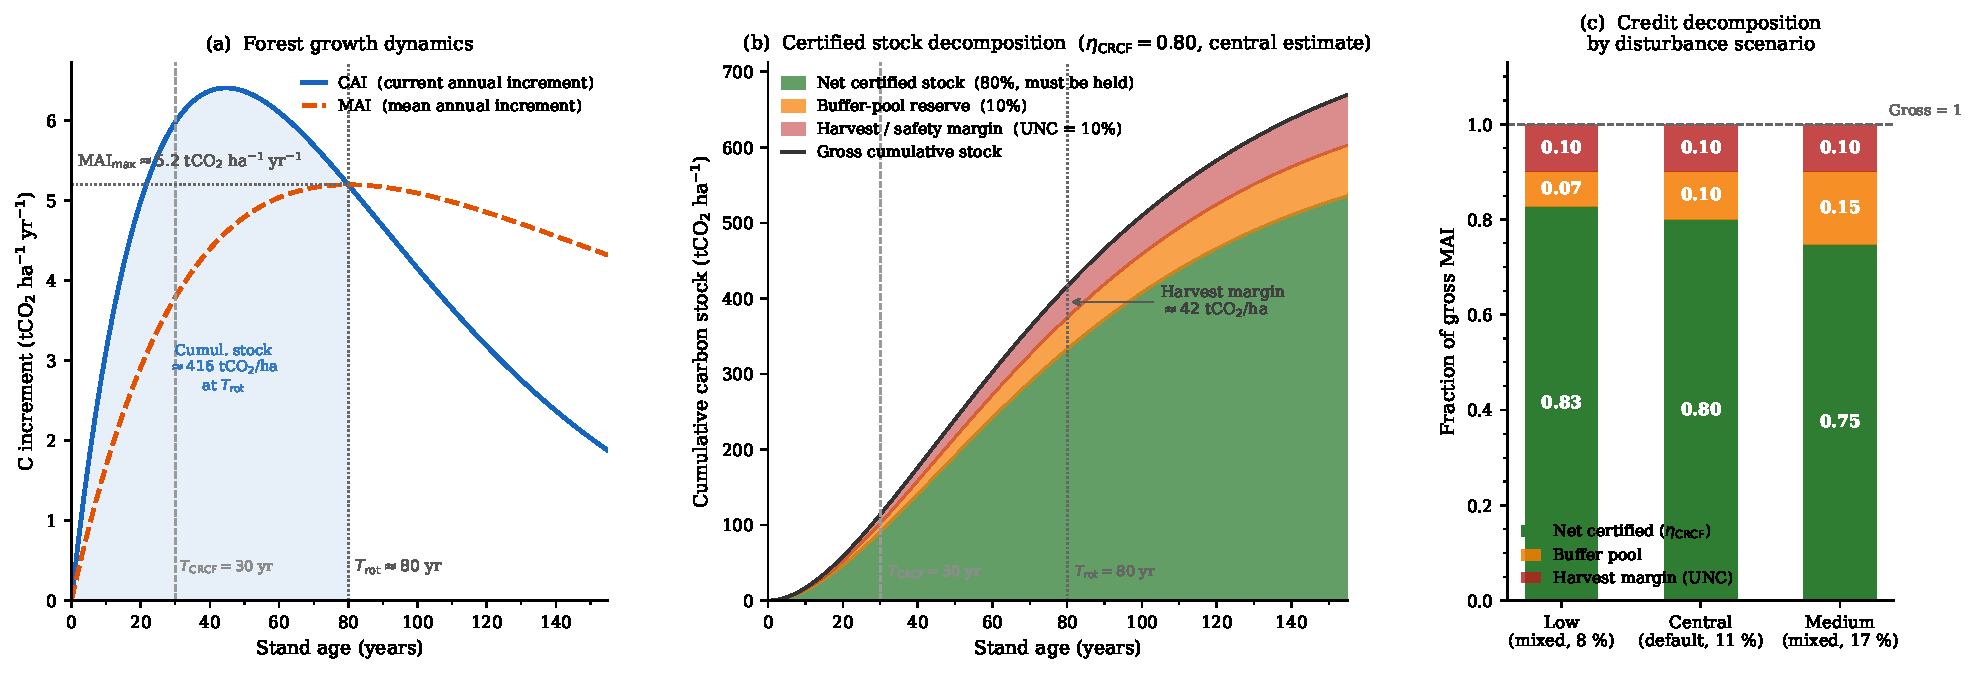
\includegraphics[width=\textwidth]{figures/mai_crcf_explained.pdf}
  \caption{%
    \textbf{Forest growth dynamics, certified stock, and CRCF credit breakdown.}
    \textit{(a)} CAI (blue) and MAI (dashed orange) for a representative
    European managed forest ($T_\text{rot}\approx80$\,yr,
    MAI$_\text{max}\approx5.2$\,tCO$_2$ ha$^{-1}$ yr$^{-1}$;
    EU median from \citealt{Pilli2024Zenodo}); dashed line: 30-yr CRCF
    activity period.
    \textit{(b)} Gross cumulative stock decomposed into net certified stock
    (green), buffer-pool reserve (orange), and harvest/safety margin (red,
    = UNC fraction, extractable without triggering reversal).
    Central estimate: $\eta_\text{CRCF}=0.80$, UNC$=10\,\%$, $r=11\,\%$.
    \textit{(c)} Same fractions for three disturbance scenarios
    (Table~7, draft delegated act, 22~Jan.~2026).}
  \label{fig:mai_crcf}
\end{figure}

% =============================================================================
\subsubsection{PyPSA-Eur implementation}
\label{sec:affo_pypsa}

Each network node~$r$ carries a \texttt{Store} on a dedicated
\texttt{co2 afforestation} bus, supplied from \texttt{co2 atmosphere} via a
monodirectional \texttt{Link} with efficiency $\eta_\text{CRCF}$
(Eq.~\ref{eq:crcf_efficiency}).  The \texttt{Store} \texttt{e\_nom\_max}~$= \Pi_r$
(Eq.~\ref{eq:node_potential}) is the annual CDR ceiling; capital cost is the
annualised per-hectare investment divided by the growth rate
(Section~\ref{sec:affo_pypsa_comparison}). Both methods are available via
\texttt{afforestation[potential\_type]} (\texttt{``density''}: \citealt{Fernandes2026};
\texttt{``growth''}: this work).

\paragraph{LP formulation.}
The link \texttt{p\_nom} is fixed to the seasonal peak rate at full deployment:
\begin{equation}
    p_{\mathrm{nom},r}
    = \Pi_r \cdot
      \frac{\displaystyle\max_{t}\, w_{m(t),r}}
           {\displaystyle\sum_{t} w_{m(t),r}}
    \quad [\mathrm{tCO_2\,h^{-1}}]
    \label{eq:pnom_cap}
\end{equation}
with \texttt{p\_min\_pu}$\,{=}\,0$ and \texttt{p\_max\_pu}$\,{=}\,1$.
The optimiser therefore allocates the annual removal $e_{\mathrm{nom,opt},r}
\le \Pi_r$ freely across the year, subject only to this instantaneous cap.
Encoding the seasonal profile as time-varying \texttt{p\_min\_pu}$(t)
{=}$ \texttt{p\_max\_pu}$(t)$ (the previous formulation) would prescribe the
temporal shape exactly but densely populates the LP constraint matrix
(${\sim}8760 \times N$ nonzero entries vs.\ a single scalar), increasing
solve time without affecting the optimised store capacity.
Capping \texttt{p\_nom} at the seasonal peak (Eq.~\ref{eq:pnom_cap}) prevents
degenerate single-hour spikes while preserving the correct annual total.

\paragraph{Seasonal post-processing.}
Before temporal plotting, \texttt{afforestation\_postprocess.py} redistributes
link flows and store state of charge according to the GPP weights:
\begin{equation}
    \Delta e_r(t)
    = \frac{w_{m(t),r}}{\displaystyle\sum_{t'} w_{m(t'),r}}
      \cdot e_{\mathrm{nom,opt},r},
    \qquad
    p_{0,r}(t) = \Delta e_r(t)\,/\,\eta_{\mathrm{CRCF}}
    \label{eq:postprocess}
\end{equation}
This is called automatically from \texttt{plot\_balance\_timeseries.py} and
\texttt{plot\_heatmap\_timeseries.py} prior to computing any time-series
statistics; all energy-system quantities are unchanged.

% =============================================================================
\subsubsection{Results and Validation}
\label{sec:affo_results}

The computed rotation-averaged sequestration rates range from
\SIrange{2.1}{12.6}{tCO_2\per ha\per yr} across 114~NUTS-2 regions with
direct Pilli data, with a European median of \SI{5.2}{tCO_2\per ha\per yr}
and mean of \SI{5.5}{tCO_2\per ha\per yr}. These values are consistent with
the \SIrange{5}{15}{tCO_2\per ha\per yr} range reported for temperate European
afforestation in the literature \citep{Nabuurs2013, Avitabile2024}.

As a validation case, the five Danish NUTS-2 regions yield rates of
\SIrange{3.9}{5.8}{tCO_2\per ha\per yr}, with a national average of
approximately \SI{5.1}{tCO_2\per ha\per yr}. This is in reasonable
agreement with the \SI{6.5}{tCO_2\per ha\per yr} estimated by
\citet{Fernandes2026} for a 60\%~conifer / 40\%~broadleaf species mix;
the difference is attributable to the equal-weight species averaging used
here versus an area-weighted approach giving greater weight to
higher-productivity conifer species.

Table~\ref{tab:affo_rates_sample} reports a selection of regional rates.

\begin{table}[htbp]
\centering
\caption{Rotation-averaged CO$_2$ sequestration rates for selected NUTS-2
regions. $\bar{T}$: mean rotation age across productive forest types;
$n$: number of productive forest types in the 50/50 con/broad blend.
Dashes indicate regions filled via the spatial fallback cascade
(Section~\ref{sec:affo_nuts2_coverage}), for which $\bar{T}$ and $n$
are not defined at NUTS-2 level.}
\label{tab:affo_rates_sample}
\sisetup{round-mode=places, round-precision=1}
\begin{tabular}{
    l
    l
    S[table-format=2.1]
    l
    l
}
\toprule
{Country} & {NUTS-2} &
{Rate [\si{tCO_2\,ha^{-1}\,yr^{-1}}]} &
{$\bar{T}$ [yr]} & {$n$} \\
\midrule
Austria   & AT21  & 6.8  & 47  & 8   \\
Belgium   & BE35  & 6.8  & 34  & 7   \\
Czechia   & CZ01  & 5.2  & 48  & 4   \\
Denmark   & DK01  & 5.8  & 39  & 7   \\
Denmark   & DK05  & 3.9  & 39  & 7   \\
Finland   & FI1D  & 3.4  & --- & --- \\
France    & FR42  & 5.4  & --- & --- \\
Germany   & DE21  & 7.2  & 34  & 8   \\
Ireland   & IE01  & 7.1  & --- & --- \\
Italy     & ITH5  & 5.6  & 40  & 14  \\
Poland    & PL42  & 6.7  & --- & --- \\
Romania   & RO21  & 6.0  & 28  & 9   \\
Sweden    & SE11  & 4.4  & 100 & 4   \\
Sweden    & SE33  & 2.1  & 32  & 4   \\
\bottomrule
\end{tabular}
\end{table}

Figure~\ref{fig:affo_monthly_nodes} shows the resulting monthly sequestration
rates aggregated to the 50-node PyPSA-Eur network. The seasonal pattern is
consistent with expectations: rates are near zero across most of Europe in
winter (December--February), rise sharply in spring, peak in June--July for
temperate and boreal nodes, and decline again in autumn. Southern nodes
(Iberian Peninsula, Italy, Greece) exhibit a broader active season and a
relatively flatter seasonal cycle, reflecting the year-round photosynthetic
activity captured by the FluxCom GPP climatology in Mediterranean climates.
The highest monthly rates (\(\approx \SI{1.5}{tCO2 ha^{-1} month^{-1}}\))
occur in central European nodes during peak summer, consistent with the
high rotation-averaged MAI values reported for Germany, Austria, and Ireland
in Table~\ref{tab:affo_rates_sample}.

\begin{figure}[htbp]
    \centering
    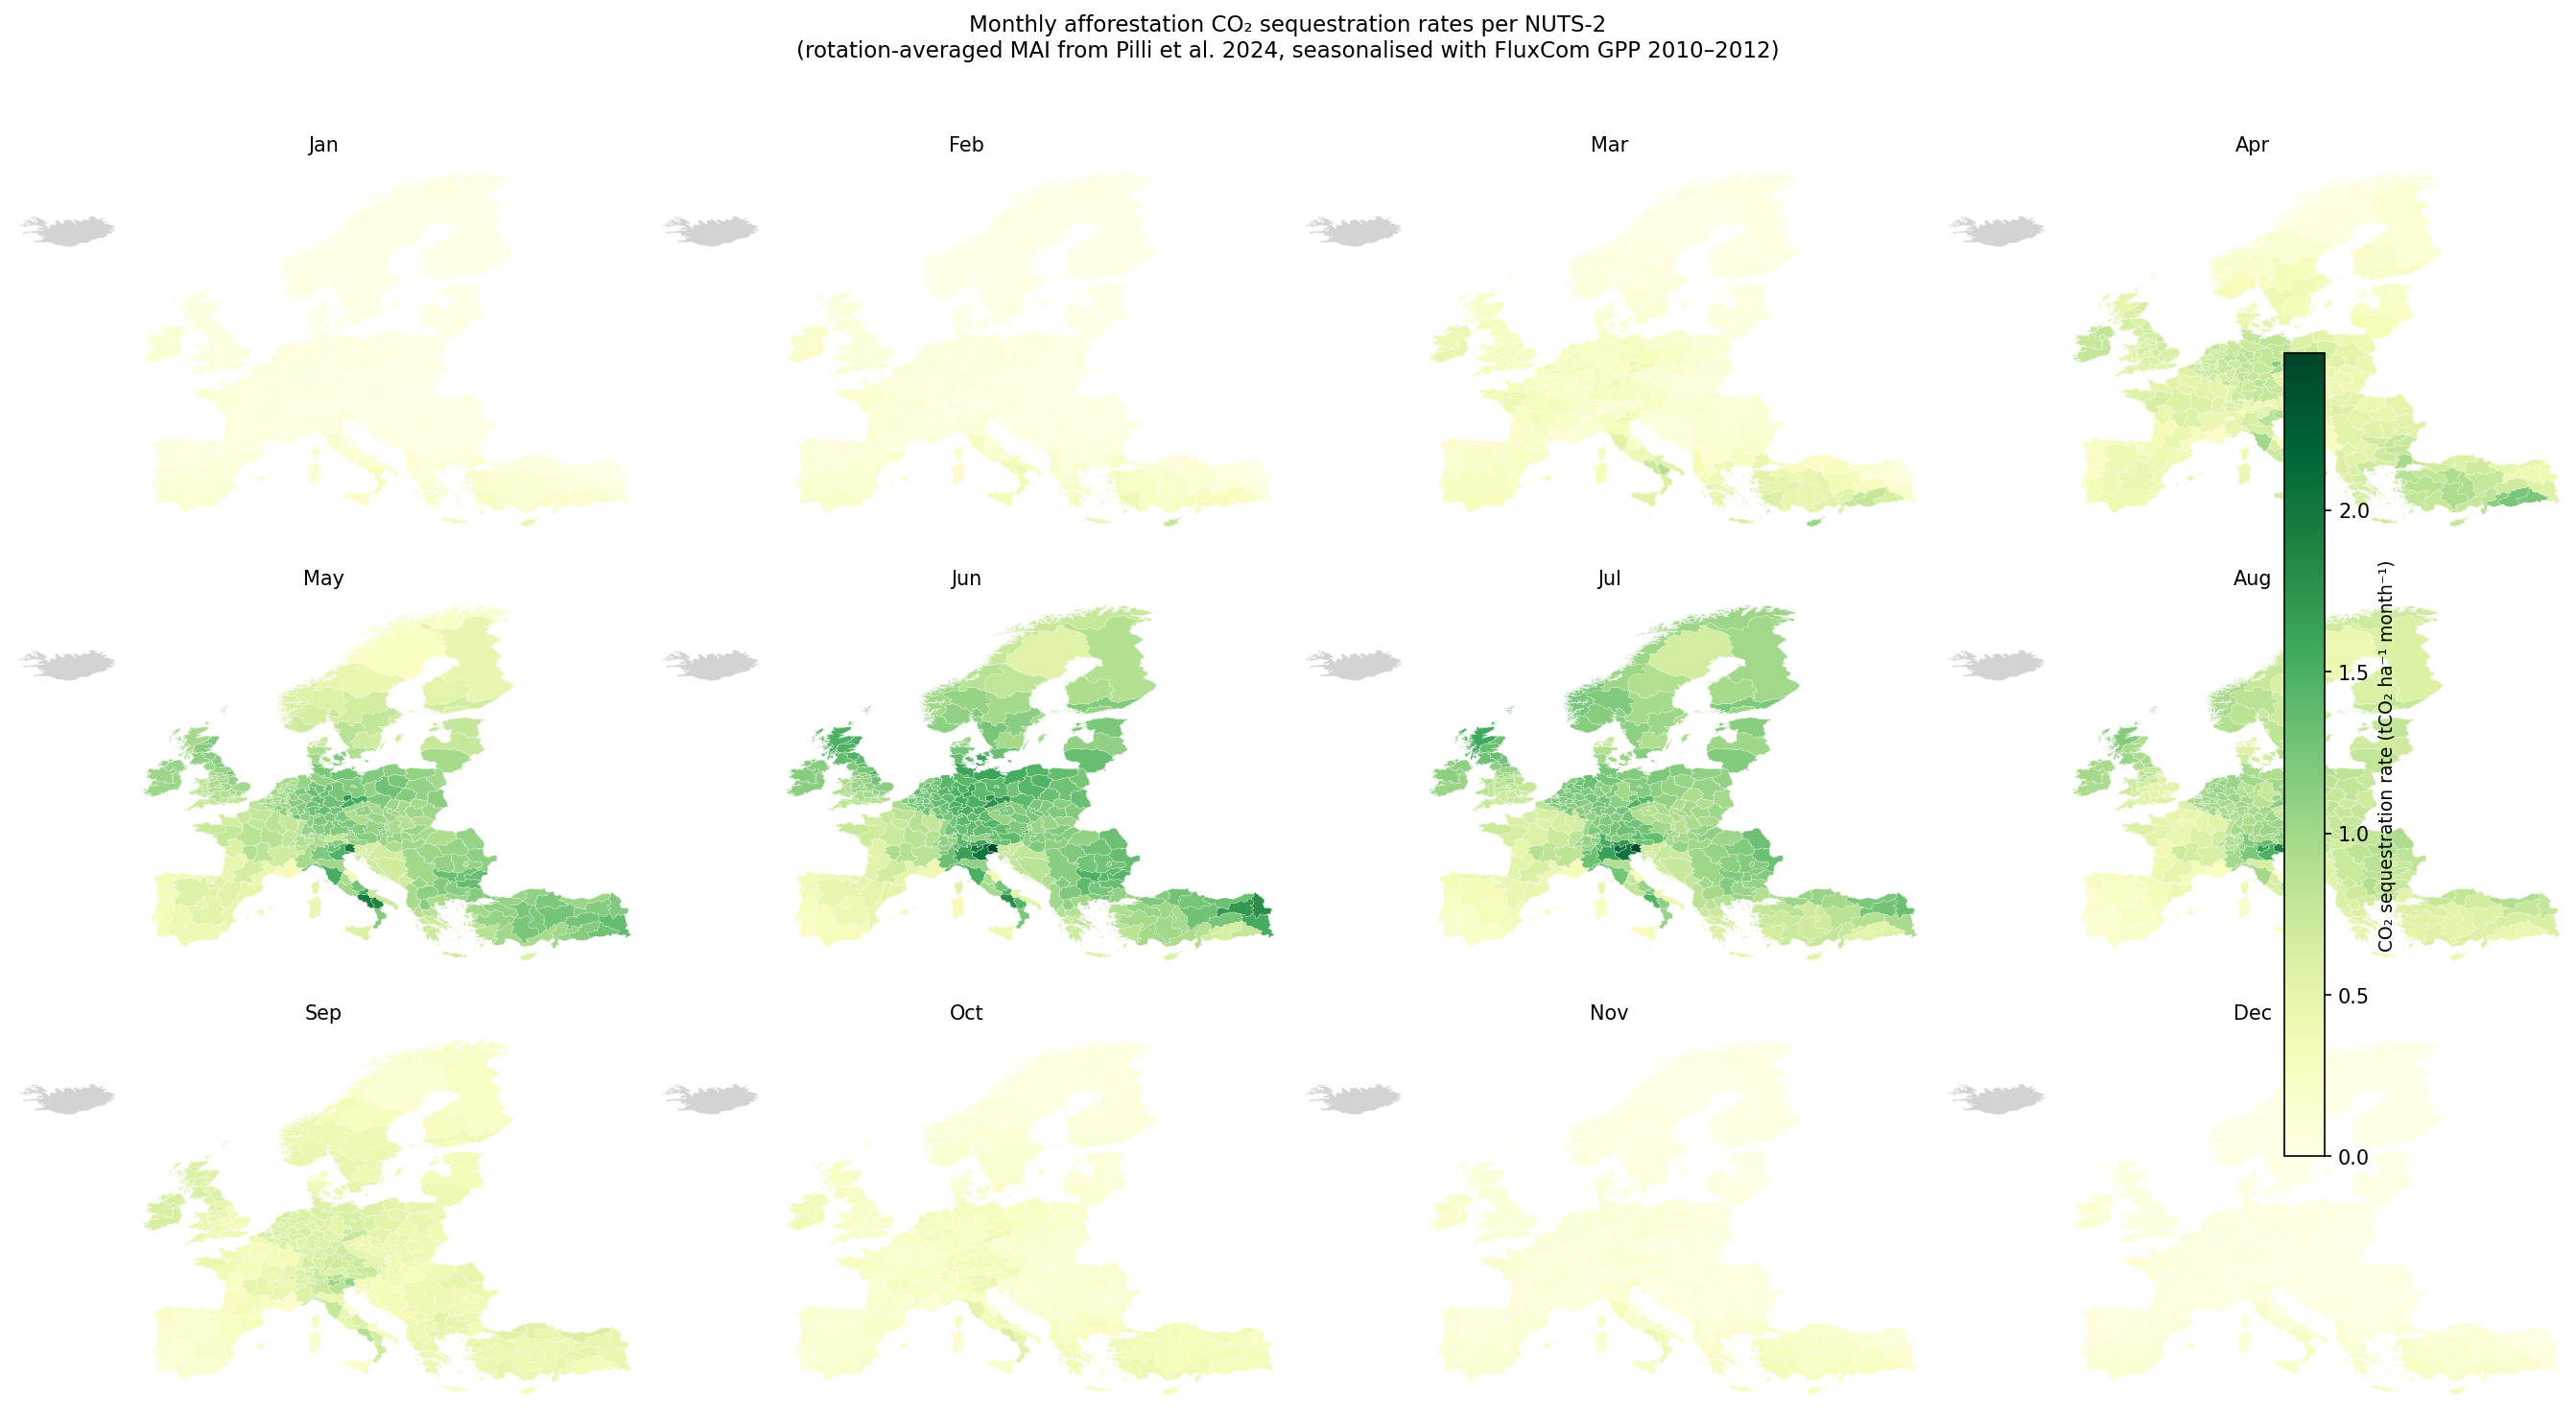
\includegraphics[width=\textwidth]{figures/fig_seasonal_map.png}
    \caption{Monthly afforestation CO$_2$ sequestration rates per NUTS-2 regions
    [\si{tCO2 ha^{-1} month^{-1}}].
    Each panel shows one calendar month; node colours reflect the product of
    the rotation-averaged MAI (Section~\ref{sec:affo_mai}) and the
    GPP-derived monthly weight $w_{m,r}$ (Eq.~\ref{eq:monthly_rate}).
    The strong north--south gradient in summer activity and the near--zero
    winter rates in boreal and continental nodes are clearly visible.
    Generated by \protect\texttt{build\_afforestation\_potentials.py} in the
    PyPSA-Eur \protect\texttt{afforestation} branch.}
    \label{fig:affo_monthly_nodes}
\end{figure}

% =============================================================================
\subsubsection{Comparison with the Density-Based Method}
\label{sec:affo_comparison}

\paragraph{Density-based method (Fernandes et al.\ 2026).}
The original implementation in \citet{Fernandes2026} derives the annual CO$_2$ sequestration rate from the standing above-ground biomass density of existing forests, using the Avitabile pan-European AGB map \citep{Avitabile2024}. The intrinsic sequestration rate is:
\begin{equation}
    \tilde{r}_{\text{density}, r}
    = \frac{\rho_r}{\tau} \times f_{\text{CO}_2}
    \quad [\text{tCO}_2\,\text{ha}^{-1}\,\text{yr}^{-1}]
    \label{eq:density_rate_intrinsic}
\end{equation}
where $\rho_r$~[\si{t_{DM}\,ha^{-1}}] is the above-ground biomass density of existing forests in region~$r$, $\tau = 30$~yr is a fixed lifetime, and $f_{\text{CO}_2} = 1.83$~\si{tCO_2\,t_{DM}^{-1}} is the CO$_2$ equivalent per tonne of dry biomass. In PyPSA-Eur, this intrinsic rate is further multiplied by a dimensionless land-utilization scaling coefficient $f_{\text{land}} = 0.6$:
\begin{equation}
    r_{\text{density}, r}
    = \tilde{r}_{\text{density}, r} \times f_{\text{land}}
    \quad [\text{tCO}_2\,\text{ha}^{-1}\,\text{yr}^{-1}]
    \label{eq:density_rate}
\end{equation}
$f_{\text{land}}$ is a policy scaling parameter, not a physical property of the forest. It captures the assumption that only a fraction of the available afforestation land will actually be planted, and it is applied identically to both the growth and density methods in PyPSA-Eur. It is therefore excluded from the method comparison below, which focuses on the intrinsic CO$_2$ sequestration rates $\tilde{r}$ derived from each data source. The Avitabile dataset provides biomass density estimates primarily at NUTS-0 (country) level; sub-national NUTS-2 resolution is obtained by applying the national value uniformly to all child NUTS-2 regions. Countries absent from the Avitabile dataset (principally the Western Balkans) receive a hardcoded fallback of $\rho = 117$~\si{t_{DM}\,ha^{-1}}. The density method assigns a uniform sequestration rate across all 12 months (i.e.\ $w_{m,r} = 1/12$), without seasonal variation.

\paragraph{Data origin per NUTS-2 region.}
The spatial coverage of the two methods differs substantially, reflecting the distinct data sources and spatial resolution of their respective filling strategies.
Figure~\ref{fig:diag_nuts2_sources} shows, for each NUTS-2 region, which step of the filling logic provided the sequestration rate.

For the \emph{growth method} (left panel), the filling cascade operates at NUTS-2 resolution: regions with a direct entry in the Pilli yield-table library are coloured dark green; regions that inherited a NUTS-1 or NUTS-0 entry are progressively lighter green. Regions not covered by Pilli at any administrative level receive a distance-weighted neighbour mean (within 100~km, orange) or a country mean (dark orange). The four Western Balkans pseudo-regions (RS/AL/BA/XK) are not present in the Pilli dataset and therefore also receive a neighbour mean (orange).

For the \emph{density method} (right panel), the filling logic is simpler: all NUTS-2 regions within a country receive the single national (NUTS-0) AGB density from Avitabile (blue). Countries absent from that dataset fall back to the hardcoded $117~\si{t_{DM}\,ha^{-1}}$ value (grey). No sub-national cascade is applied.

\begin{figure}[htbp]
    \centering
    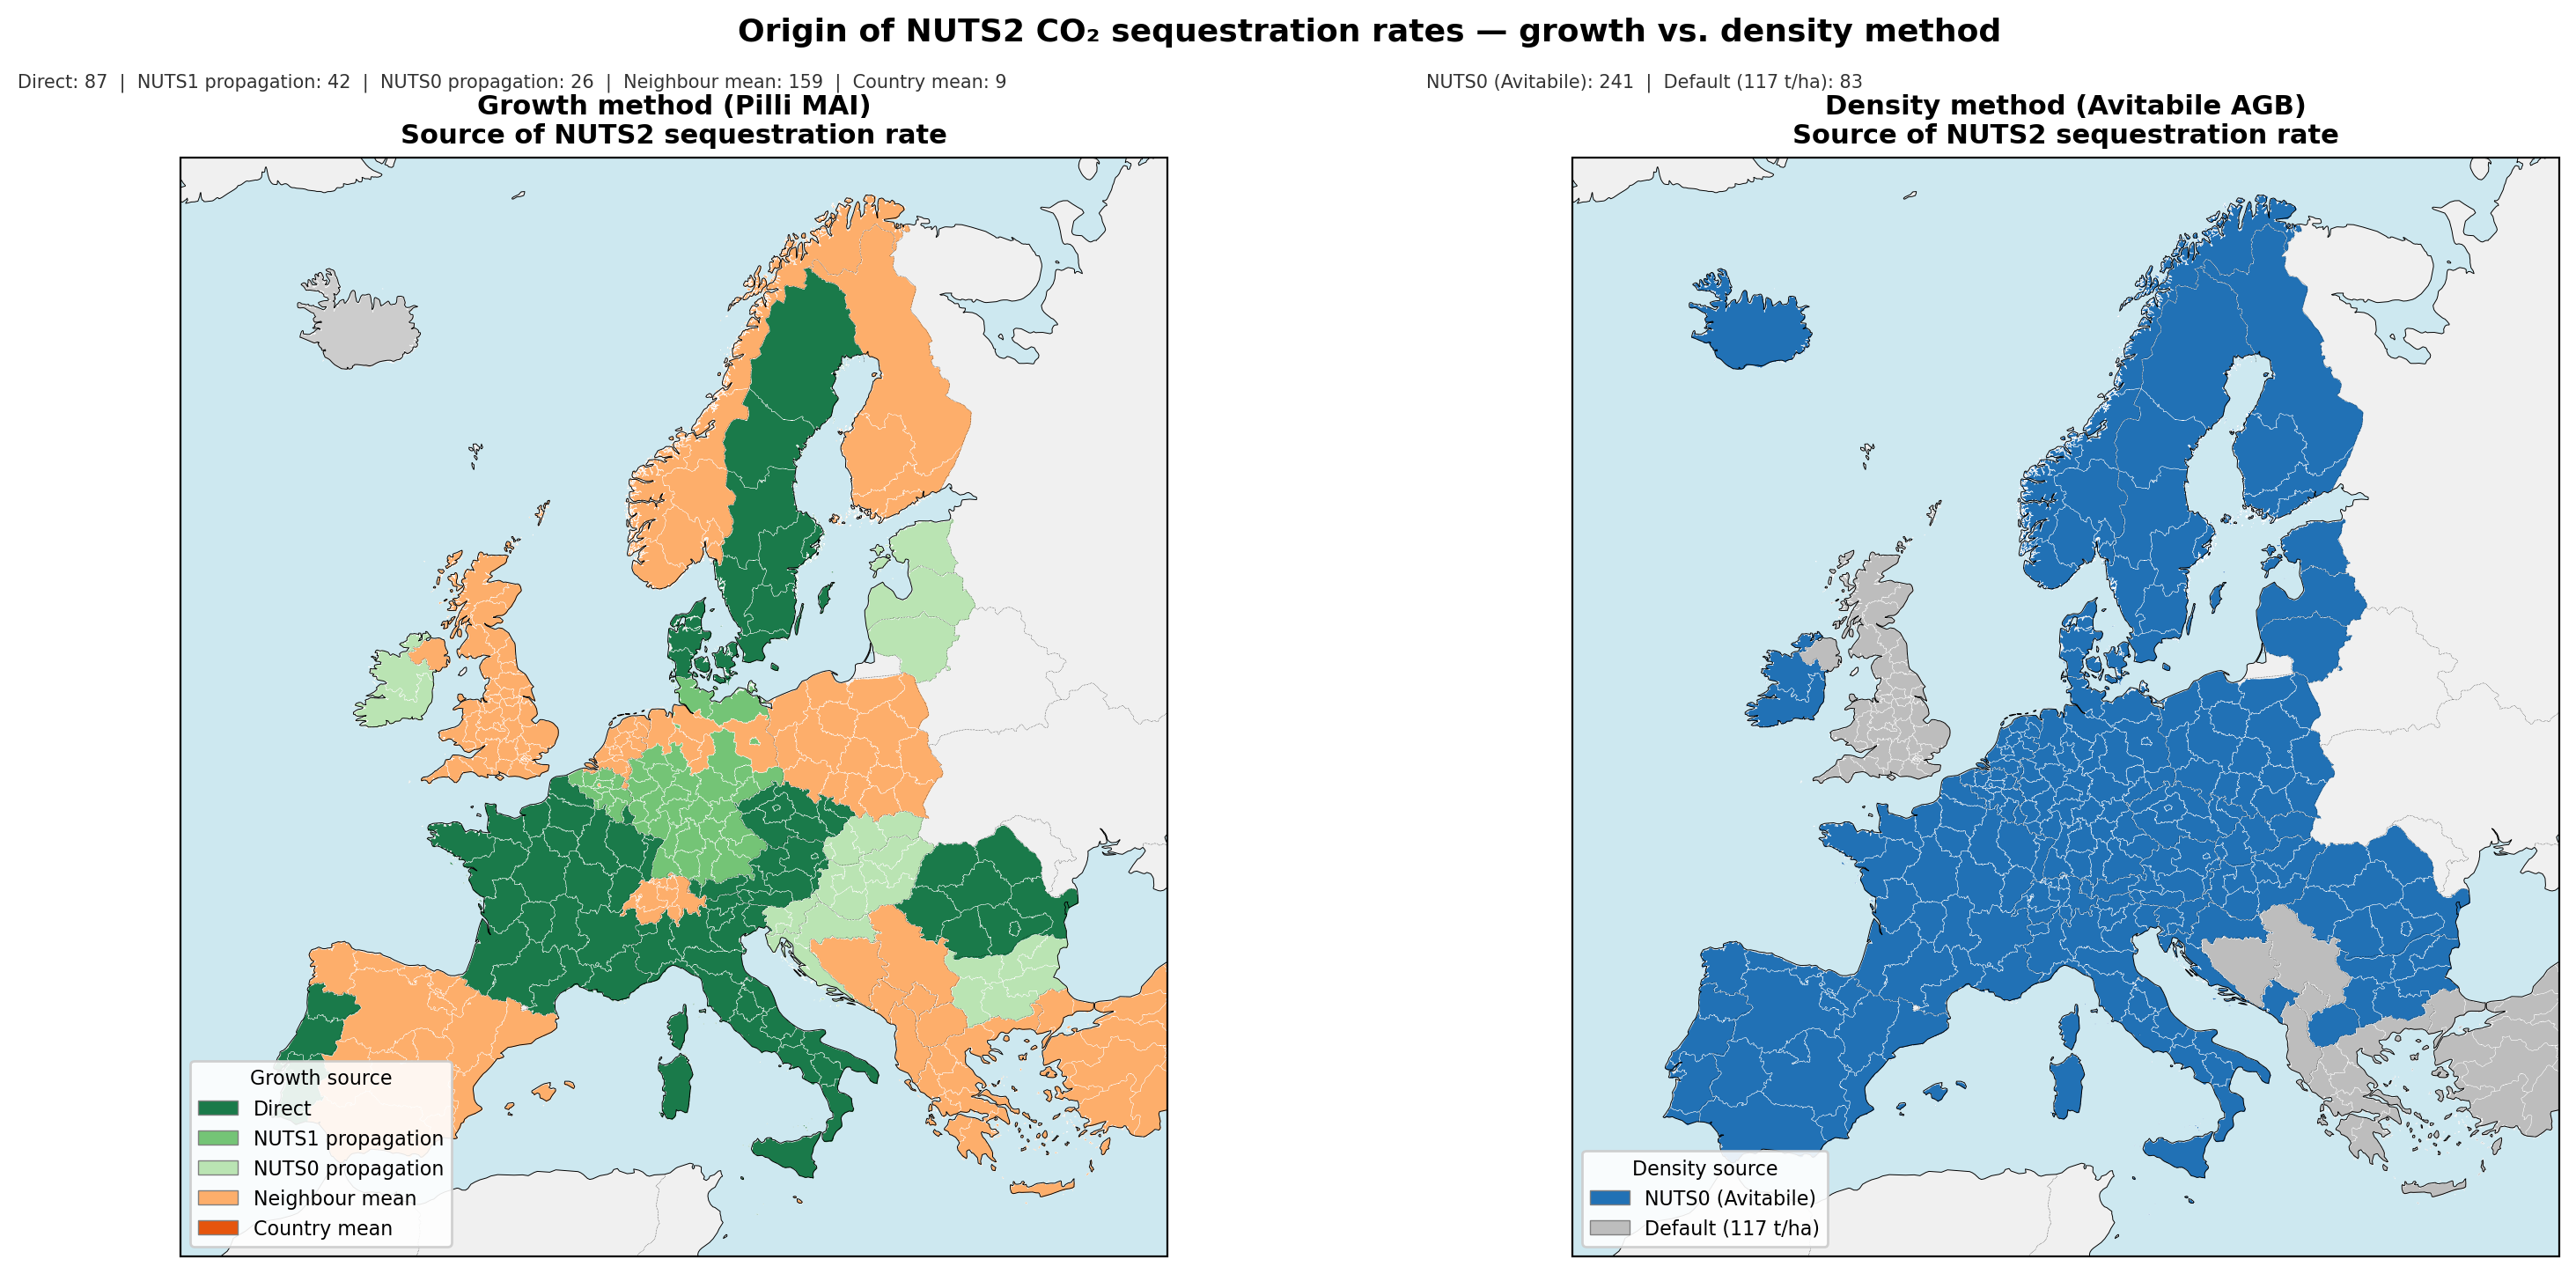
\includegraphics[width=\textwidth]{figures/fig_diag_nuts2_sources.png}
    \caption{Origin of the NUTS-2 CO$_2$ sequestration rate for each region.
    \textit{Left:} growth method (Pilli MAI). Colours indicate which step of the
    six-step filling cascade provided the rate: dark green = direct NUTS-2 entry;
    medium/light green = NUTS-1/NUTS-0 propagation; orange = 100-km neighbour mean;
    dark orange = country mean. Western Balkans pseudo-regions (RS/AL/BA/XK)
    are absent from the Pilli dataset and appear in orange (neighbour mean).
    \textit{Right:} density method (Avitabile AGB) as implemented in PyPSA-Eur.
    Blue = country-level (NUTS-0) AGB density from Avitabile; grey = hardcoded
    fallback (117~\si{t_{DM}\,ha^{-1}}) for countries absent from the dataset,
    including the Western Balkans pseudo-regions.
    No sub-national spatial cascade is applied in the density method.}
    \label{fig:diag_nuts2_sources}
\end{figure}

\paragraph{Comparison of annual sequestration rates.}
Figure~\ref{fig:method_comparison_maps} shows the spatial distribution of annual CO$_2$ sequestration rates for both methods across all NUTS-2 regions, and the signed difference (growth minus density). The density-method rates shown are the intrinsic values $\tilde{r}_{\text{density}}$ (without the $f_{\text{land}} = 0.6$ scaling coefficient), enabling a direct comparison of the underlying forest productivity data. The growth-based rates vary at NUTS-2 resolution reflecting local forest composition and management, while the density-based rates are uniform within each country. Because $\tilde{r}_{\text{density}}$ is higher than the scaled value applied in PyPSA-Eur by a factor of $1/0.6 \approx 1.67$, the density method tends to exceed the growth method in large parts of southern and eastern Europe.

Notable differences emerge for several countries. Croatia (\texttt{HR}) has a substantially lower growth rate (${\approx}\SI{3.8}{tCO_2\,ha^{-1}\,yr^{-1}}$) than the density method (${\approx}\SI{6}{tCO_2\,ha^{-1}\,yr^{-1}}$), reflecting a predominantly low-BCEF conifer mix in the Pilli library. Finland (\texttt{FI}) and Sweden (\texttt{SE}) show higher growth rates in the south and lower in the boreal north, a spatial gradient that is invisible to the density method. Portugal (\texttt{PT}) and several southern European countries exhibit higher density-method rates, reflecting high standing biomass stock that does not translate into equally high annual increments.

\begin{figure}[htbp]
    \centering
    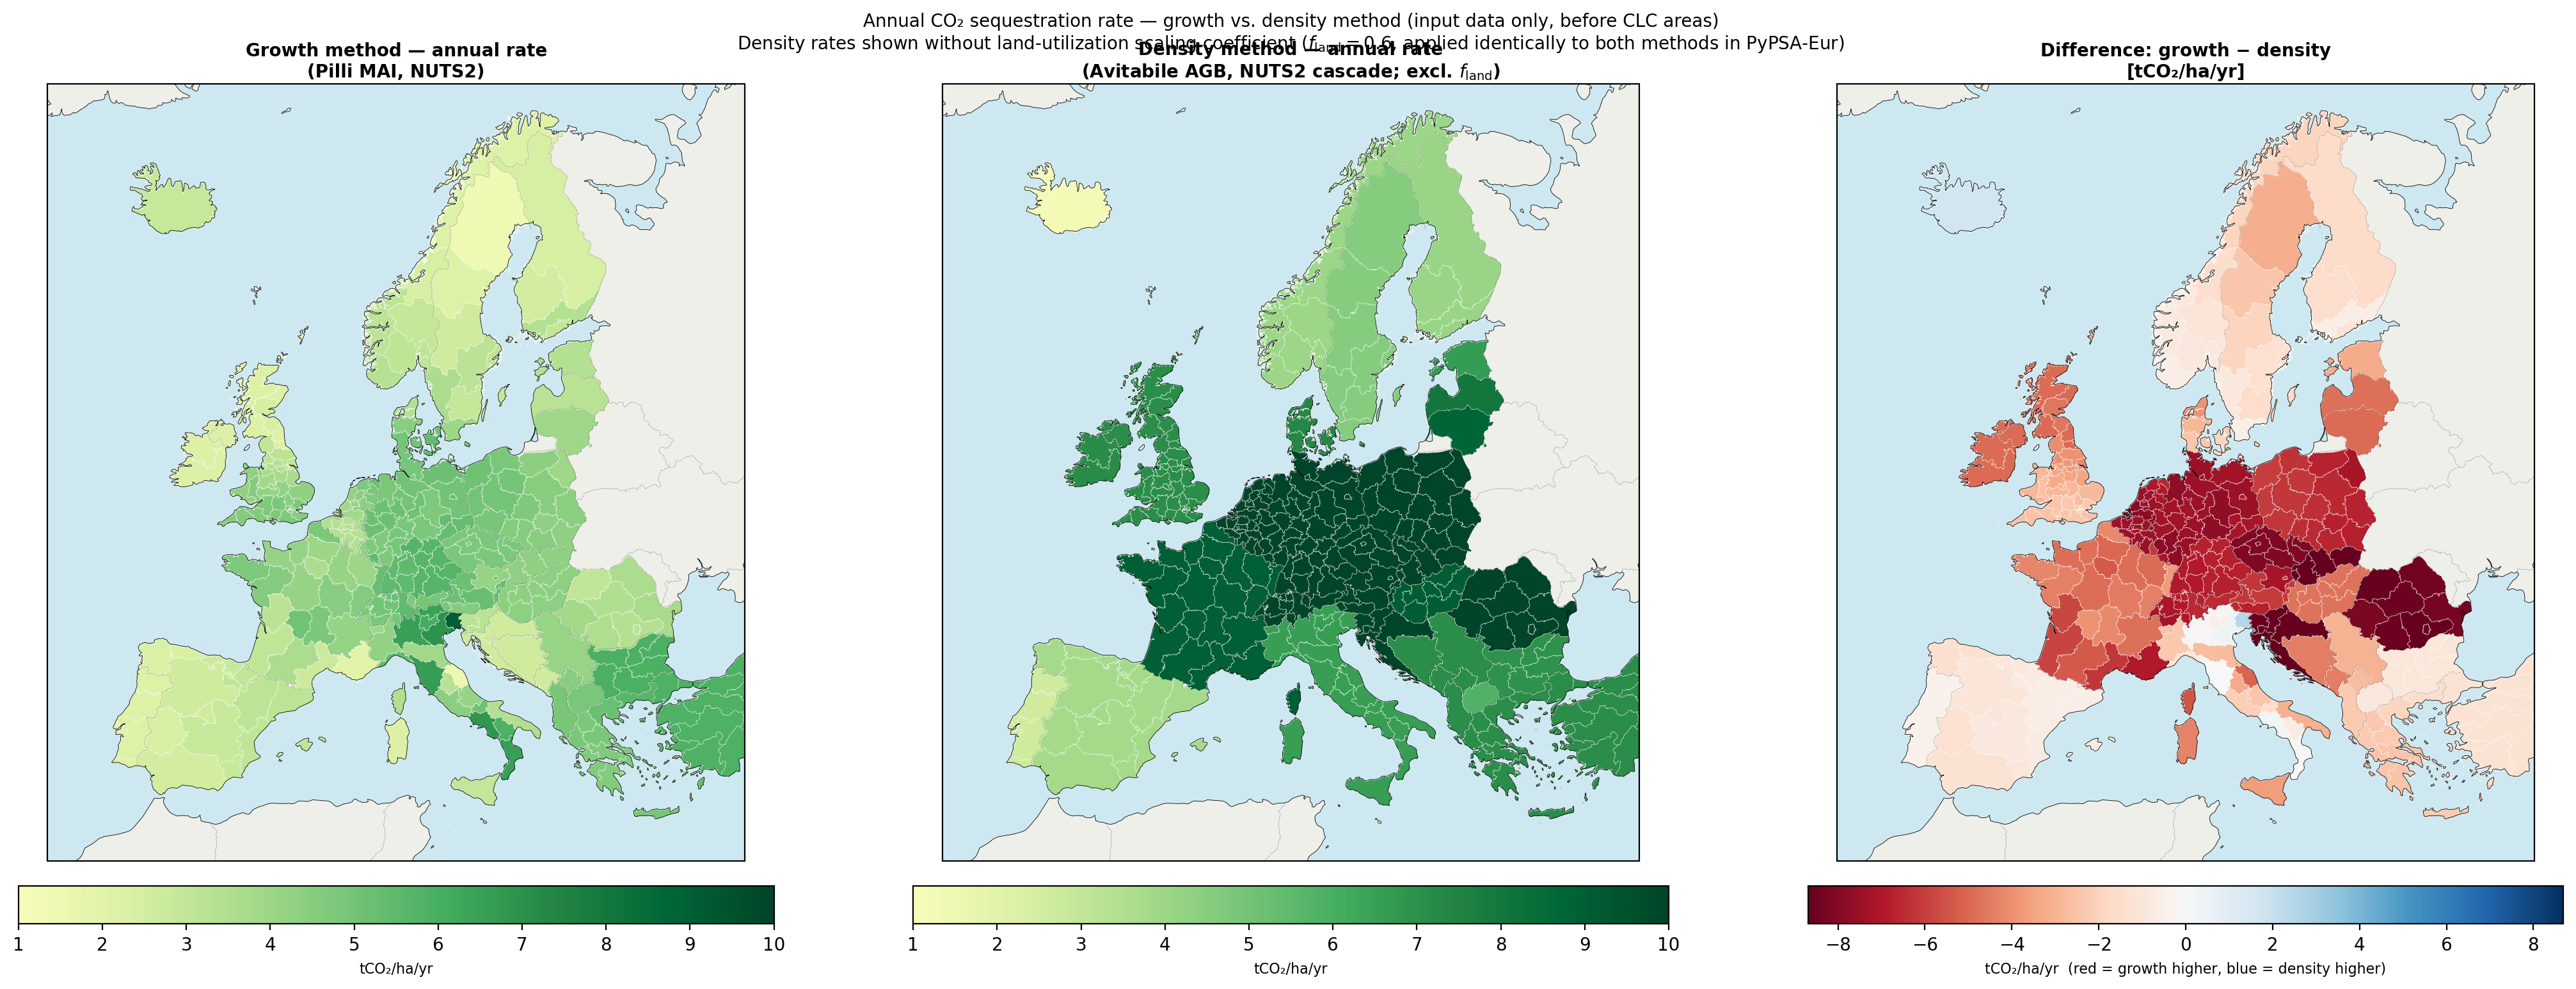
\includegraphics[width=\textwidth]{figures/fig_method_comparison_maps.png}
    \caption{Annual CO$_2$ sequestration rates [\si{tCO_2\,ha^{-1}\,yr^{-1}}] at NUTS-2 resolution.
    \textit{Left:} growth method (Pilli MAI, this work).
    \textit{Centre:} intrinsic density-method rate $\tilde{r}_{\text{density}}$
    (Avitabile AGB, \citealt{Fernandes2026}; Eq.~\ref{eq:density_rate_intrinsic}),
    uniform within each country; the land-utilization scaling coefficient
    $f_{\text{land}} = 0.6$ (Eq.~\ref{eq:density_rate}) is excluded to allow
    a like-for-like comparison of the underlying forest productivity data.
    \textit{Right:} signed difference (growth $-$ density); diverging colour scale centred at zero.}
    \label{fig:method_comparison_maps}
\end{figure}

\paragraph{Comparison of seasonal profiles.}
Figure~\ref{fig:method_comparison_seasonal} compares the monthly sequestration profiles derived from each method. The growth method follows the GPP-driven seasonal cycle, with strong summer peaks and near-zero winter rates in northern and continental regions. The density method has no seasonal variation by construction (flat line at annual rate / 12). For southern European regions, the seasonal amplitude from the growth method is modest, reflecting a longer growing season captured by the FluxCom GPP climatology.

\begin{figure}[htbp]
    \centering
    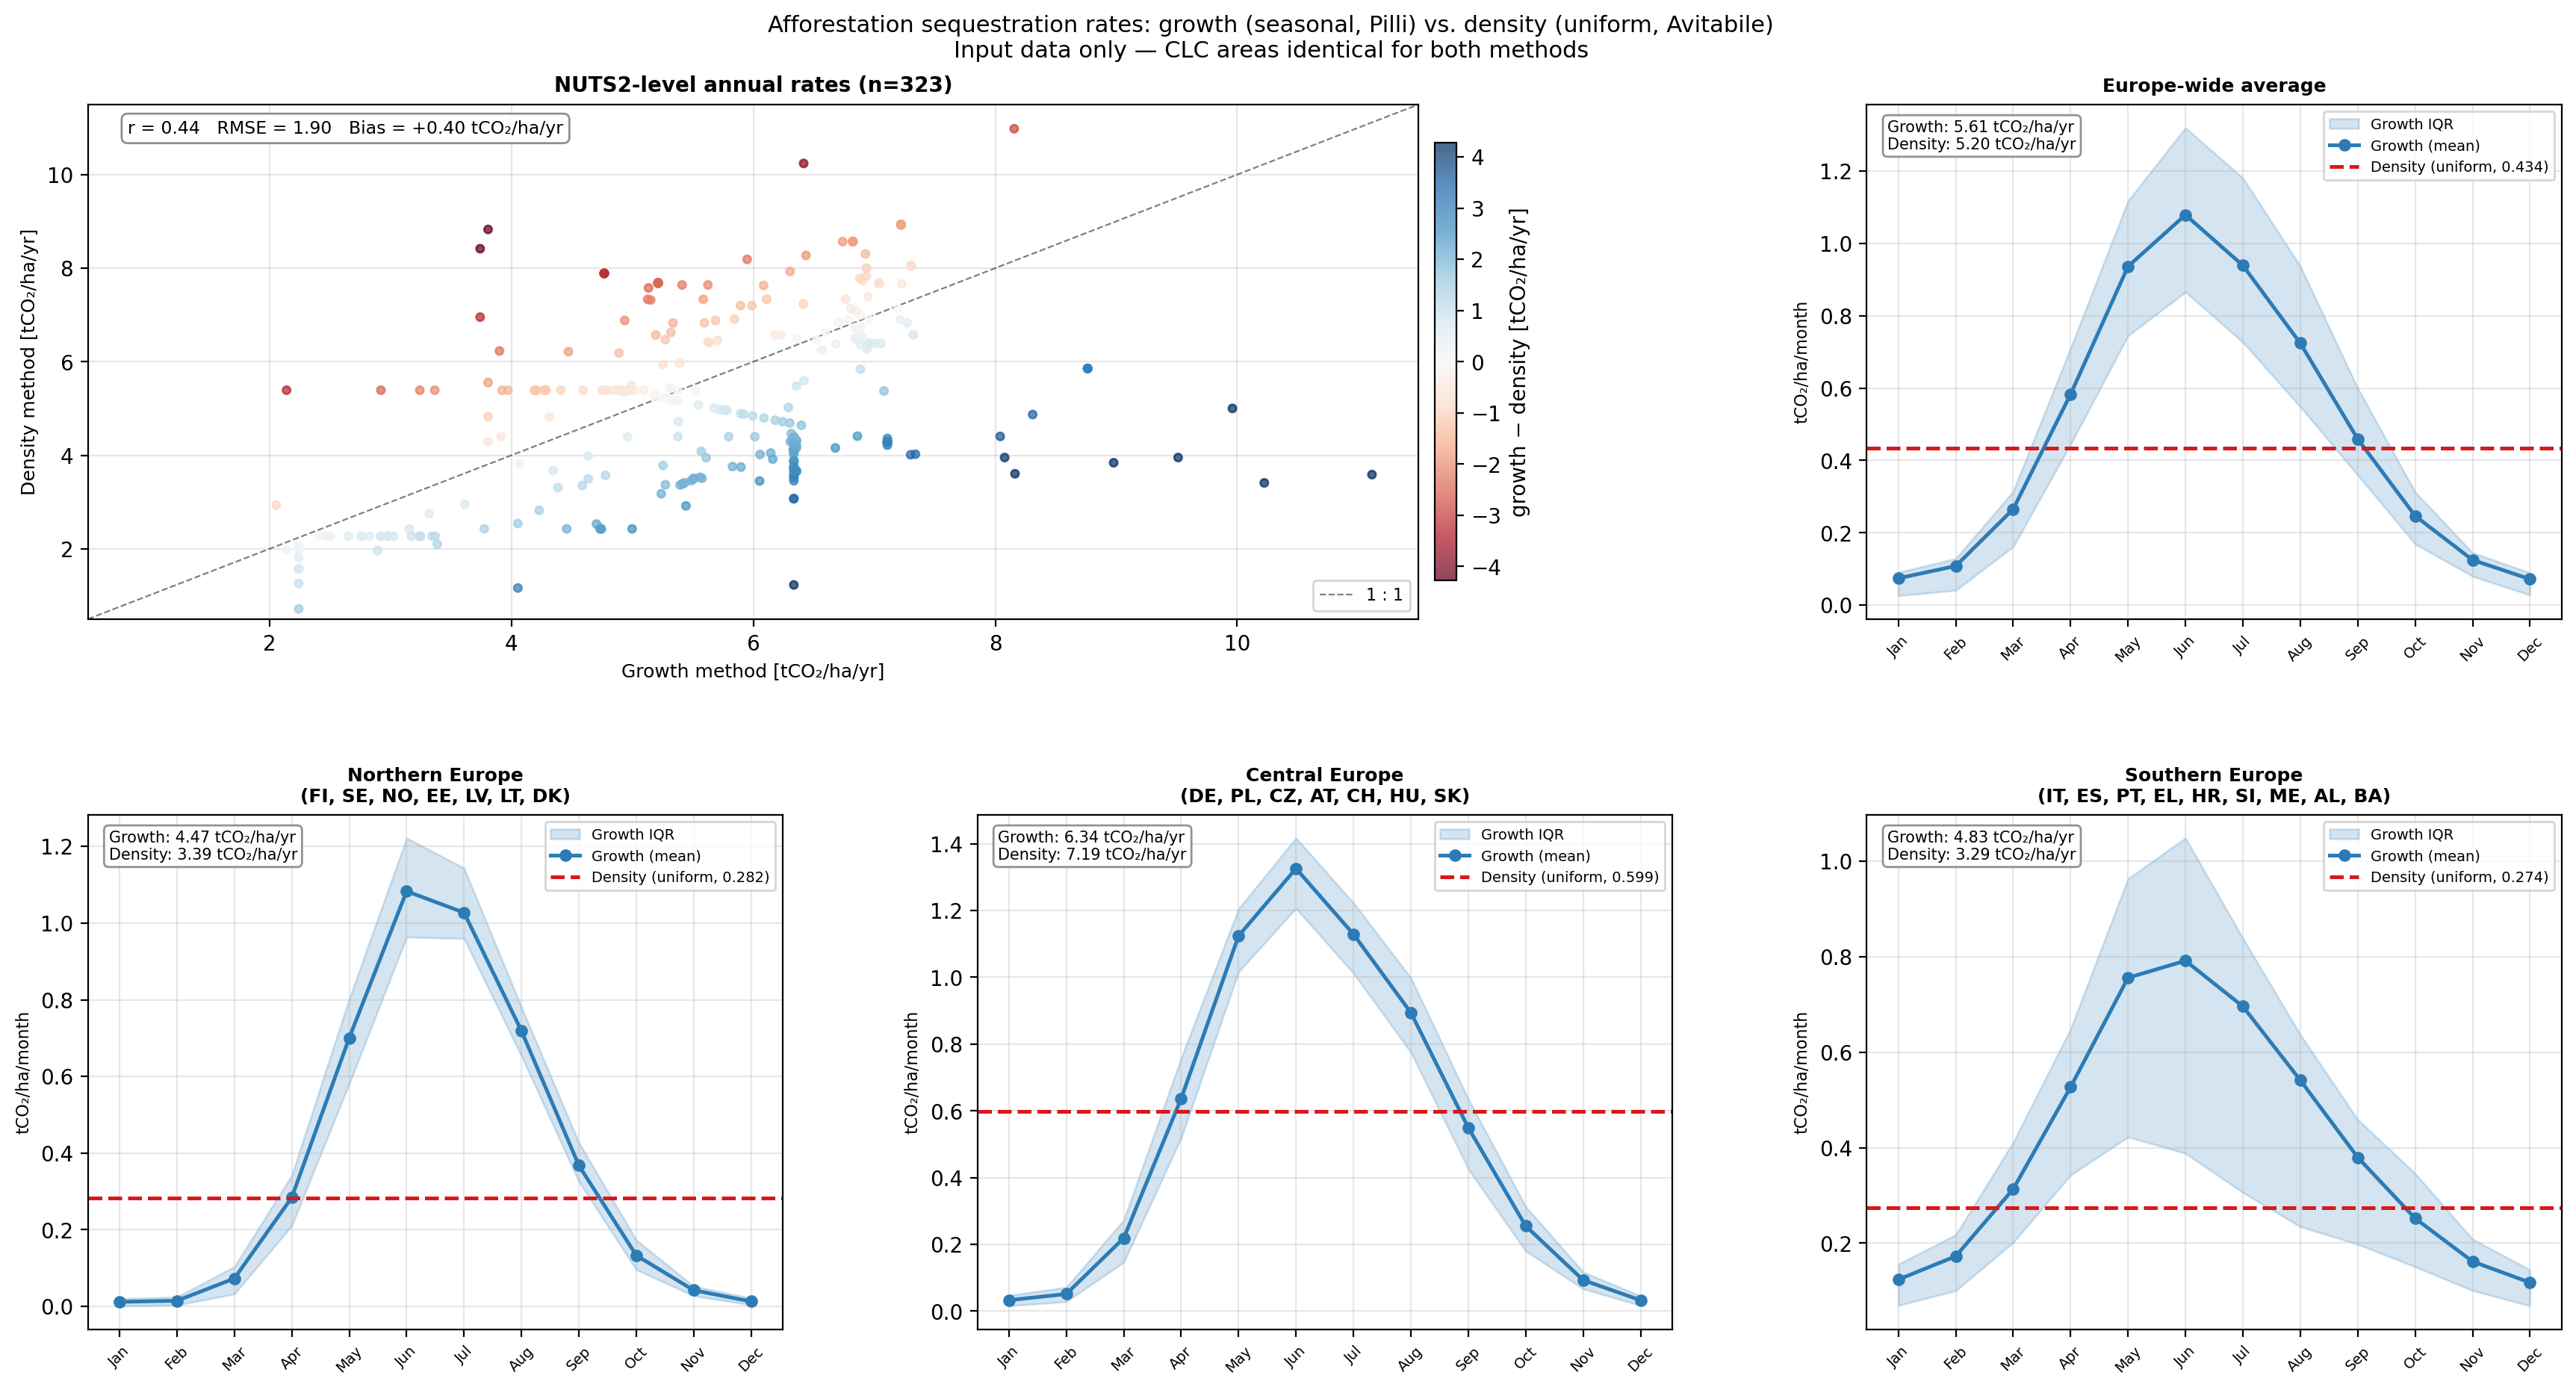
\includegraphics[width=\textwidth]{figures/fig_method_comparison_seasonal.png}
    \caption{Monthly CO$_2$ sequestration rates [\si{tCO_2\,ha^{-1}\,month^{-1}}] for the growth method
    (mean $\pm$ interquartile range across NUTS-2 regions in each macro-region; solid line)
    versus the density method (dashed flat line at annual rate / 12).
    The four panels correspond to European macro-regions spanning a north--south gradient.}
    \label{fig:method_comparison_seasonal}
\end{figure}

% =============================================================================
\subsubsection{Comparison of PyPSA-Eur Optimisation Results}
\label{sec:affo_pypsa_comparison}

To assess the quantitative impact of the two afforestation methods on system-level CDR deployment, we ran the same PyPSA-Eur configuration twice---once with the growth-based potential (Section~\ref{sec:affo_rate}) and once with the density-based potential (Section~\ref{sec:affo_comparison})---holding all other model settings identical (90 nodes, 2050 horizon, 168-h temporal resolution). Both runs use the CLC land potentials from \citet{Fernandes2026}. The density run was executed with the land-utilisation scaling $f_{\text{land}} = 0.6$. The CRCF efficiency discount $\eta = 0.8$ is applied only in the growth method, where it is implemented as the PyPSA \texttt{Link} efficiency (Section~\ref{sec:affo_pypsa}); the density method does not apply this discount.

Figure~\ref{fig:affo_pypsa_comparison_map} compares the annual afforestation potentials fed into the two optimisations. Panel~(a) shows the growth-method potential, which amounts to 99.9~\si{MtCO_2\,yr^{-1}} in total and varies at NUTS-2 resolution. Panel~(b) shows the density-method potential as used in the model (after $f_{\text{land}} = 0.6$), totalling 83.1~\si{MtCO_2\,yr^{-1}}. Panel~(c) shows the intrinsic density potential before the $f_{\text{land}}$ scaling (138.5~\si{MtCO_2\,yr^{-1}}), enabling a like-for-like comparison with the growth method on a common physical basis. The density potential is substantially higher in northern and eastern Europe where standing biomass stocks are large, but varies only at NUTS-0 (country) level. The growth method yields more spatially differentiated rates reflecting local species composition and management intensity.

\begin{figure}[htbp]
    \centering
    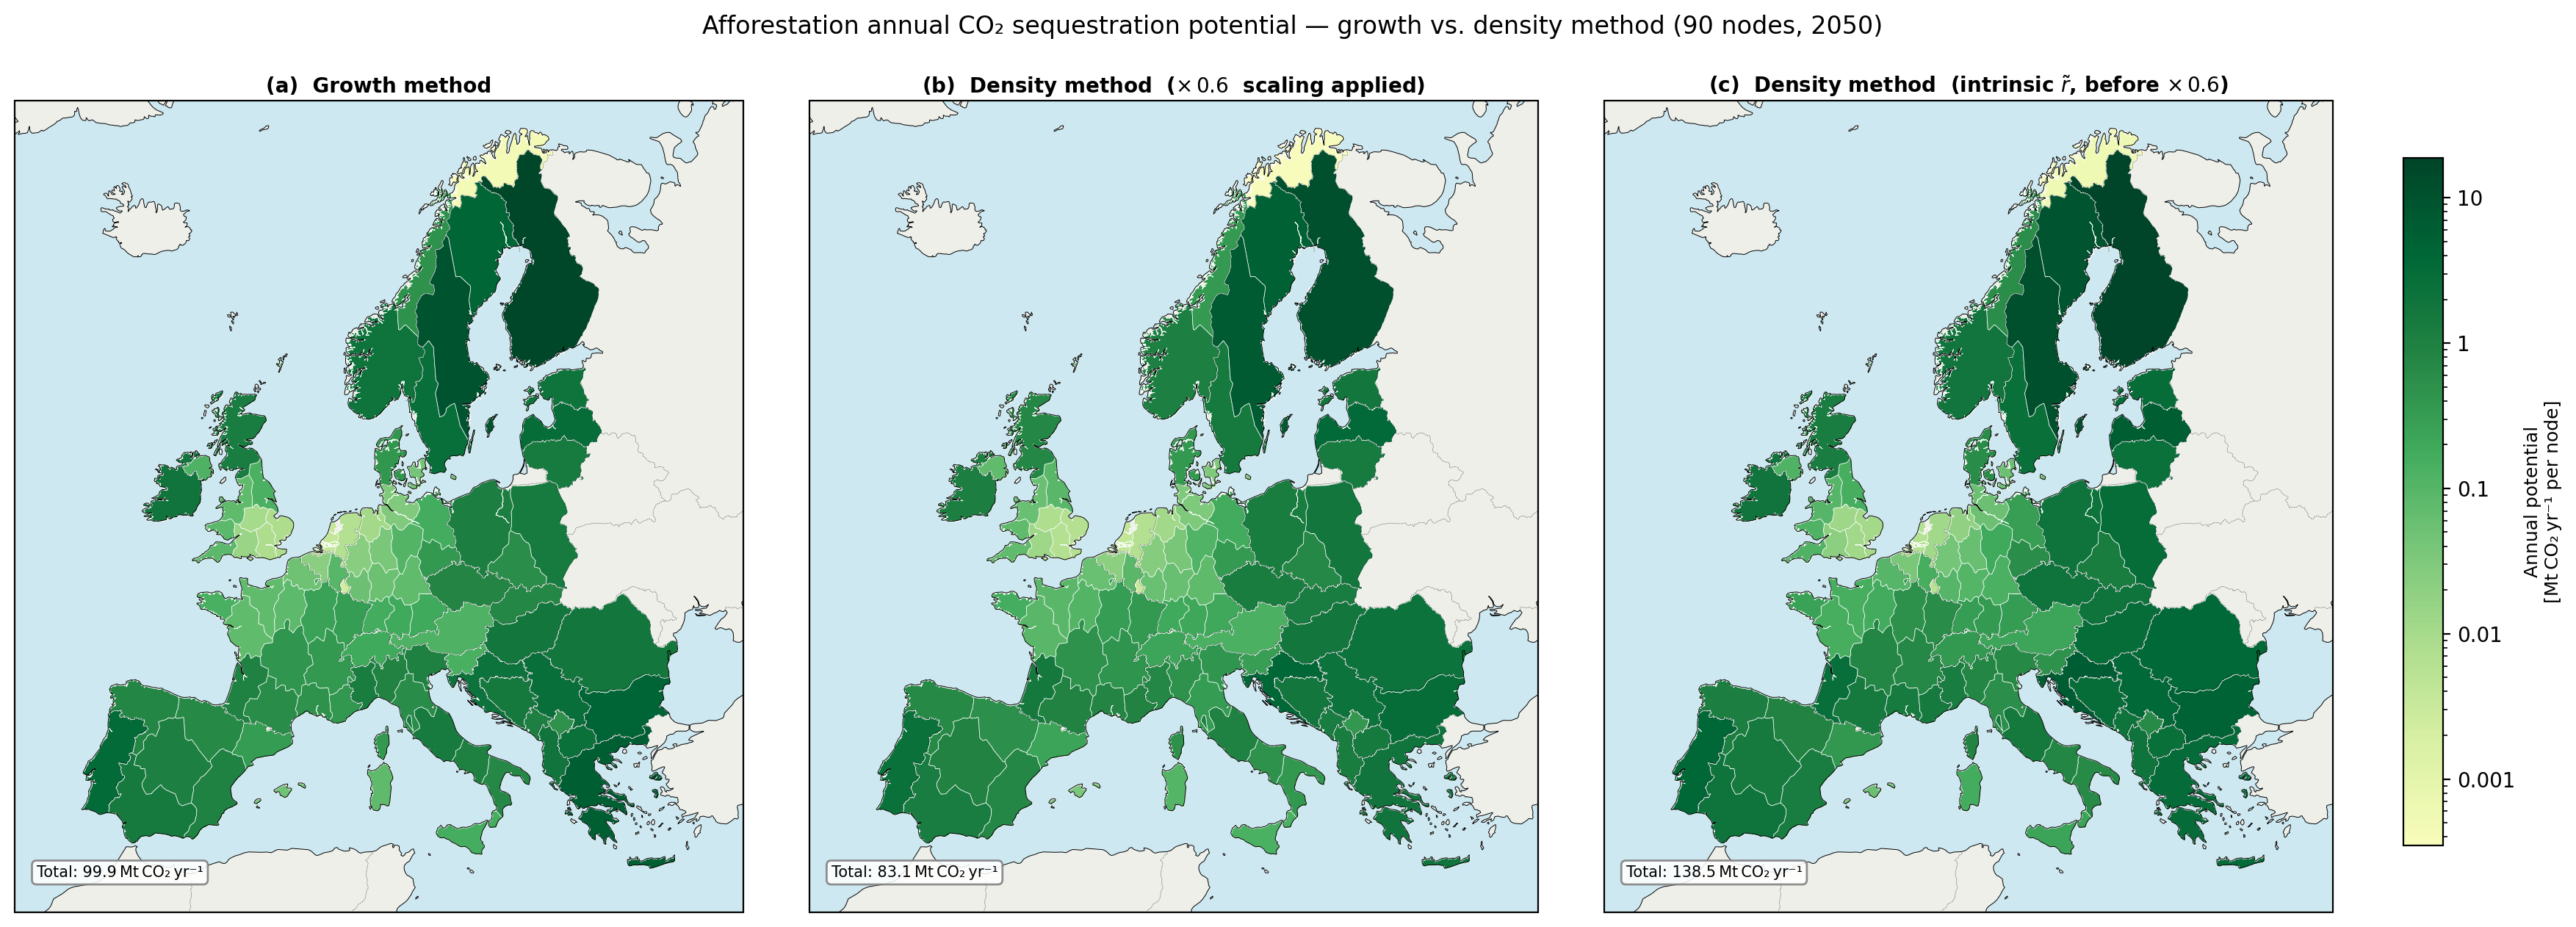
\includegraphics[width=\textwidth]{figures/fig_affo_pypsa_comparison_map.png}
    \caption{Annual afforestation CO$_2$ sequestration potential per network node
    [\si{MtCO_2\,yr^{-1}}] for three scenarios.
    (a)~Growth method (Pilli MAI, this work): 99.9~\si{MtCO_2\,yr^{-1}} total.
    (b)~Density method with land-utilisation scaling $f_{\text{land}}=0.6$
    (as used in the optimisation): 83.1~\si{MtCO_2\,yr^{-1}} total.
    (c)~Density method intrinsic rate $\tilde{r}_{\text{density}}$
    (Eq.~\ref{eq:density_rate_intrinsic}), before $f_{\text{land}}$ scaling:
    138.5~\si{MtCO_2\,yr^{-1}} total.
    All panels share the same logarithmic colour scale.}
    \label{fig:affo_pypsa_comparison_map}
\end{figure}

With the growth method, the optimizer deploys 92.0~\si{MtCO_2\,yr^{-1}} of credited CDR (92\% of the available potential), leaving 8\% unused in small or low-rate growth nodes---north of Sweden where rotation time (hence MAI) is very long (100 years), or south of France and Portugal where existing forests available for afforestation register limited growth. In all these cases the cost for afforestation rises above 500 EUR/tCO2. With the density method, the model fully saturates the scaled potential (83.1~\si{MtCO_2\,yr^{-1}}, 100\% utilisation across all nodes), as all density-method nodes carry a uniform rate that makes them equally attractive.

Figure~\ref{fig:affo_pypsa_comparison_country} shows the country-level breakdown of potentials and CDR deployment. The largest contributions in both runs come from Finland, Sweden, France, and Romania. The density method shows higher intrinsic potentials in the Baltic states and the Balkans (driven by high standing biomass stocks), while the growth method gives relatively higher rates in France and Germany where the Pilli yield-table data indicate productive managed forests.

\begin{figure}[htbp]
    \centering
    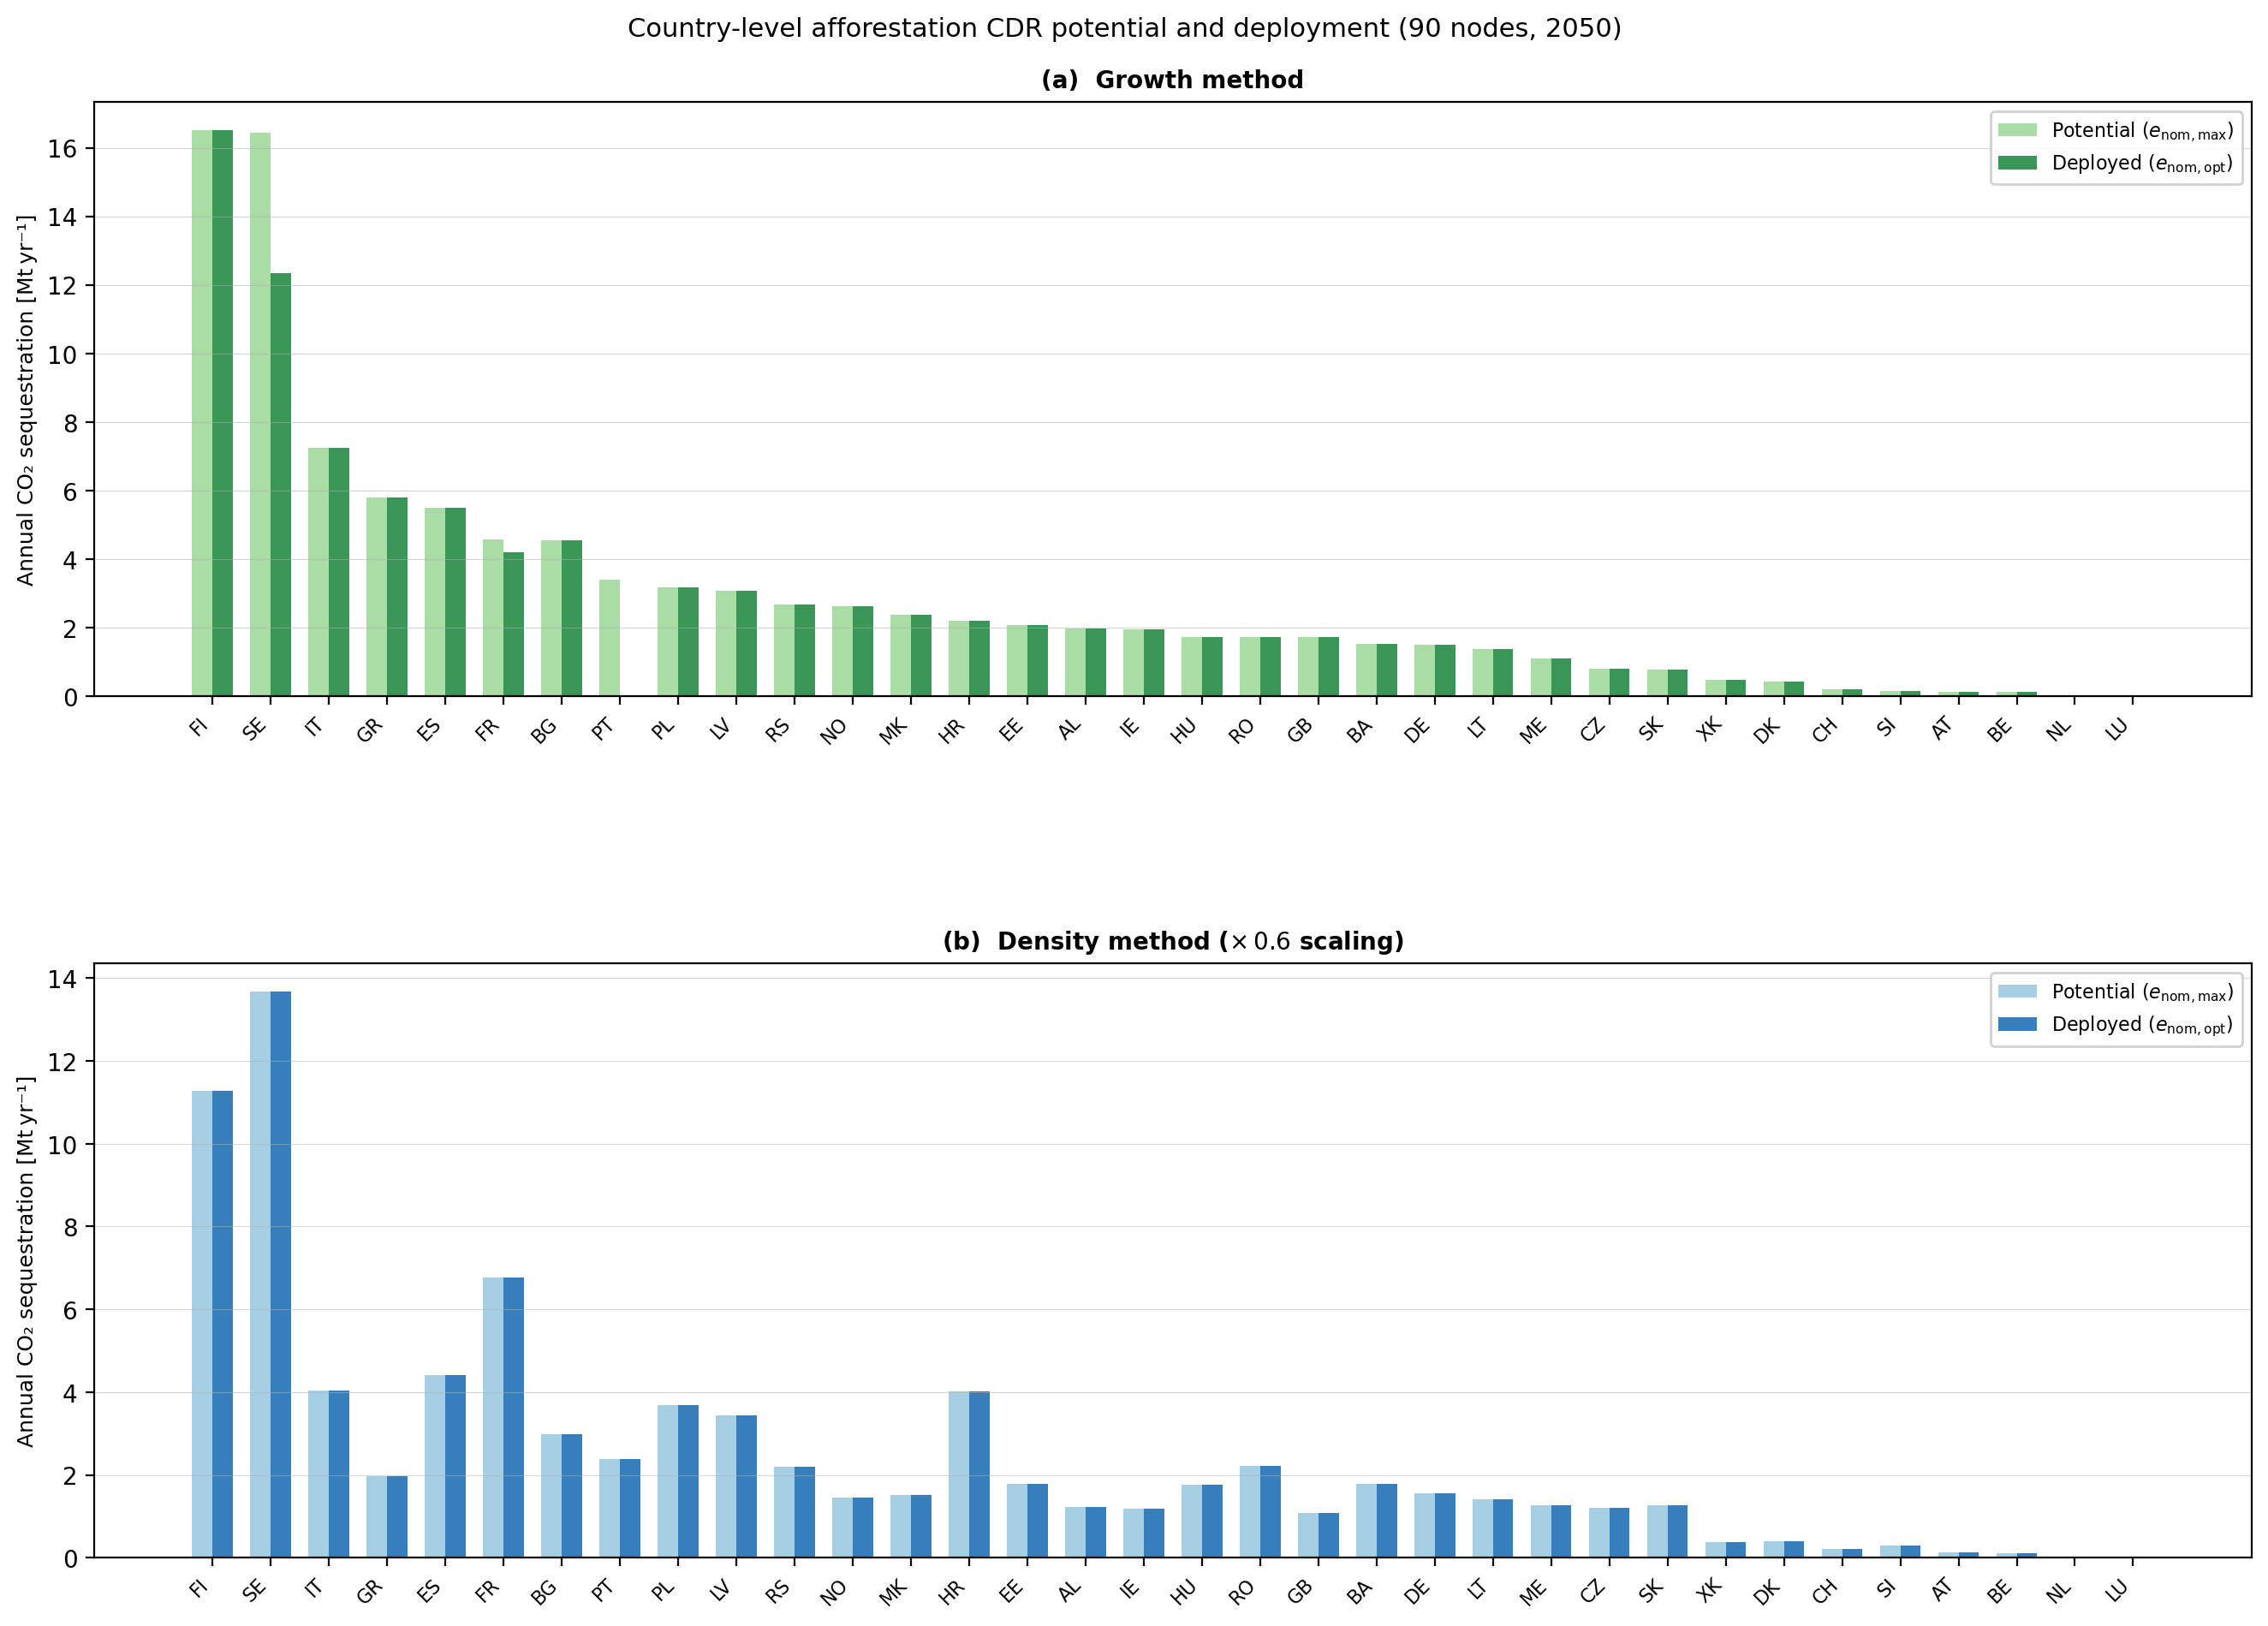
\includegraphics[width=\textwidth]{figures/fig_affo_pypsa_comparison_country.png}
    \caption{Country-level available potential ($e_{\mathrm{nom,max}}$, lighter shade)
    and optimally deployed potential ($e_{\mathrm{nom,opt}}$, darker shade)
    for the growth method (top, green) and the density method with $f_{\text{land}}=0.6$
    scaling (bottom, blue).}
    \label{fig:affo_pypsa_comparison_country}
\end{figure}

Figure~\ref{fig:ts_co2_balance} shows the CO$_2$ bus balance over the full annual time horizon
for both optimisation runs.
In the growth case (panel~a), the \texttt{co2 afforestation} component (green) follows a clear
seasonal pattern, peaking in spring and summer and declining in winter, consistent with the
GPP-derived monthly weights applied in post-processing.
In the density case (panel~b), afforestation enters as a flat, constant sink throughout the year,
reflecting the uniform $w_{m,r}=1/12$ seasonal profile of the density method.

\begin{figure}[htbp]
    \centering
    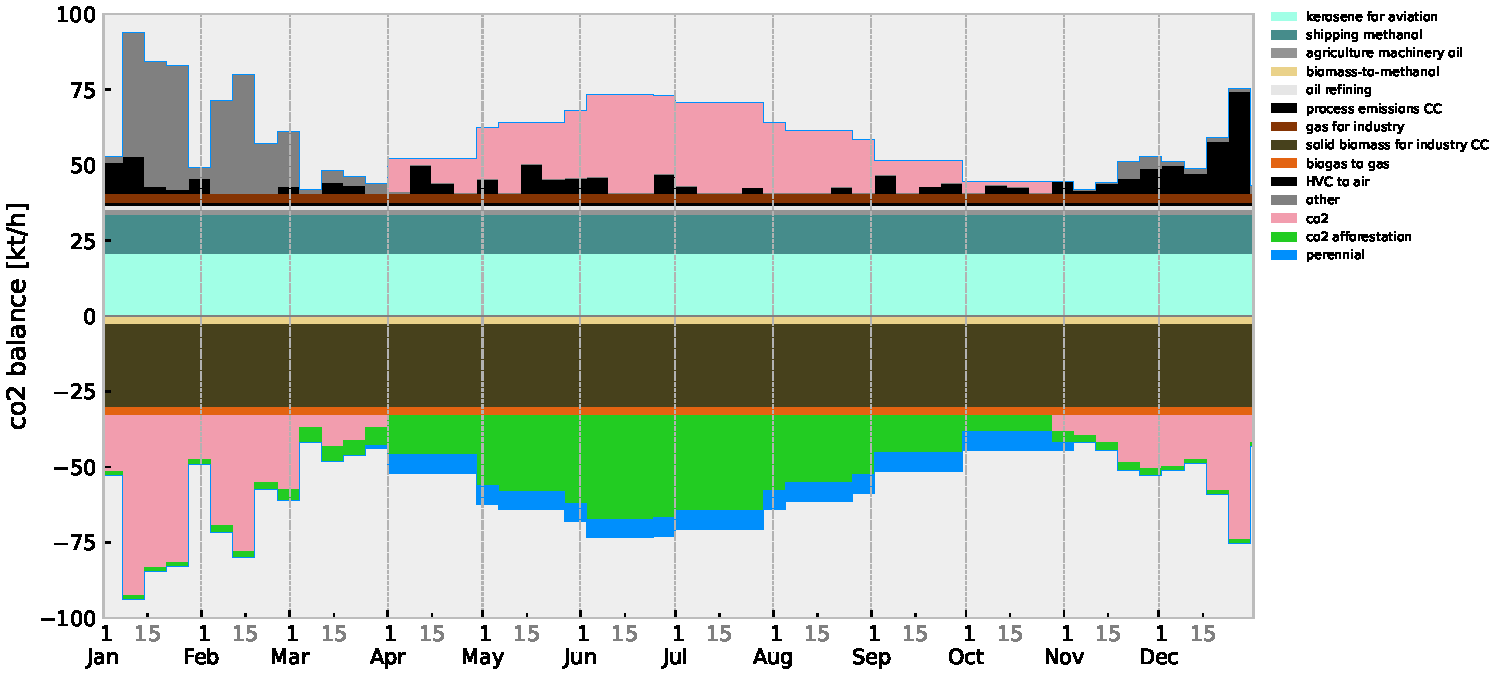
\includegraphics[width=\textwidth]{figures/ts_balance_co2_growth.pdf}\\[4pt]
    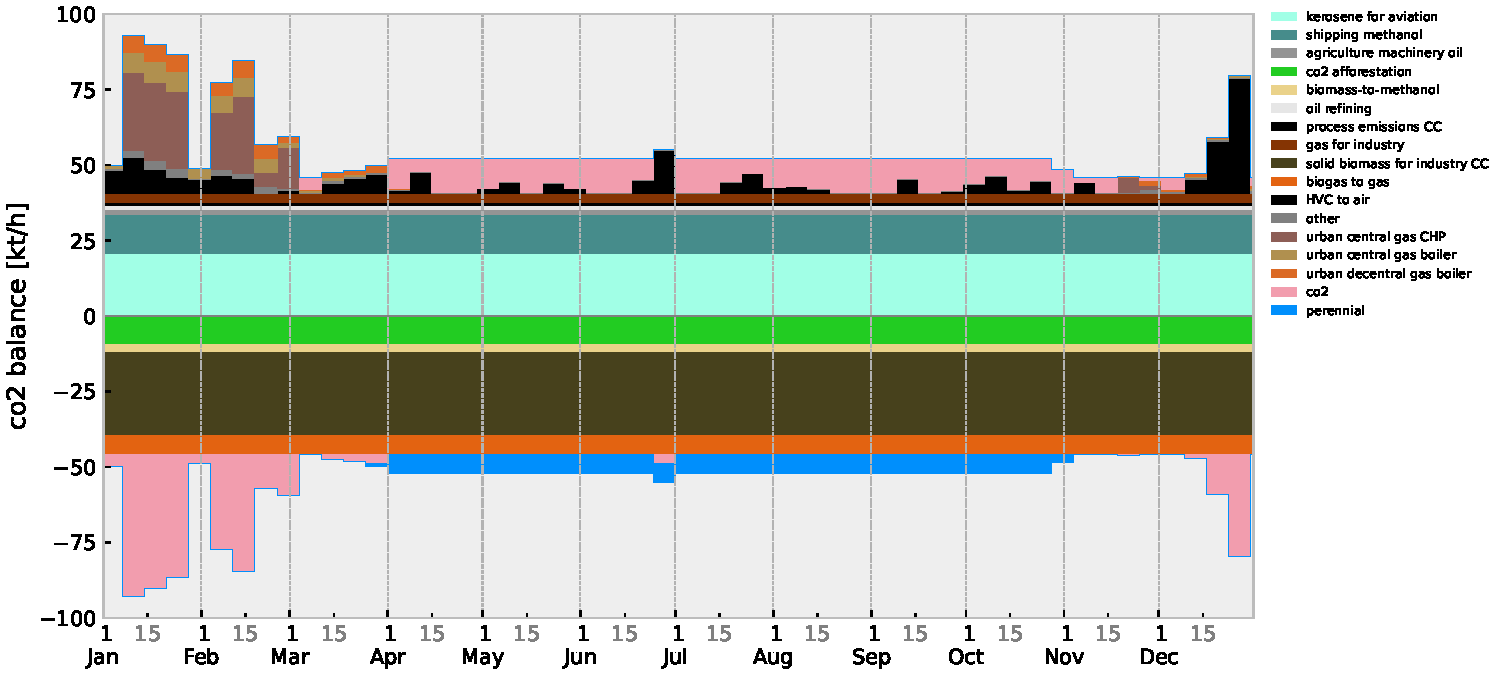
\includegraphics[width=\textwidth]{figures/ts_balance_co2_density.pdf}
    \caption{Annual CO$_2$ bus balance for the growth method (top) and the density method
    (bottom), at 168-h temporal resolution (90-node model, 2050).
    The \texttt{co2 afforestation} component is shown in green (top) and as a thin green band
    (bottom). In the growth case the seasonal signal—peaking in spring and summer—is recovered
    by \texttt{afforestation\_postprocess.py} before plotting.
    In the density case, afforestation acts as a constant sink ($w_{m,r}=1/12$).}
    \label{fig:ts_co2_balance}
\end{figure}

Table~\ref{tab:affo_pypsa_summary} summarises the key European-wide indicators from both runs. The two methods yield a near-identical system CO$_2$ price ($\approx$430~\si{EUR\,tCO_2^{-1}}) and CO$_2$-sequestration-limit shadow price ($\approx$281~\si{EUR\,tCO_2^{-1}}), indicating that the choice of afforestation method does not substantially alter the overall cost structure of the energy system at this level of temporal and spatial resolution. The main differences are: the growth method provides a larger raw potential but applies a CRCF credit discount, leaving a utilisation margin; the density method uses a smaller scaled potential but saturates it completely.

\begin{table}[htbp]
\centering
\caption{Comparison of afforestation CDR indicators from PyPSA-Eur optimisation runs
(90-node, 2050 horizon, 168-h temporal resolution).
The CRCF efficiency discount $\eta = 0.8$ is applied only in the growth method.
For the density method, potentials are reported at both the intrinsic rate $\tilde{r}$
(before $f_{\text{land}} = 0.6$) and the scaled rate used in the optimisation.}
\label{tab:affo_pypsa_summary}
\begin{tabular}{lcc}
\toprule
\textbf{Indicator} & \textbf{Growth method} & \textbf{Density method} \\
\midrule
Annual potential [\si{MtCO_2\,yr^{-1}}]                              & 99.9  & 138.5 (intrinsic) \\
Annual potential after $f_{\text{land}}=0.6$ [\si{MtCO_2\,yr^{-1}}] & 99.9\textsuperscript{a} & 83.1 \\
CRCF efficiency discount $\eta$                                       & 0.8   & --- \\
Optimised CDR [\si{MtCO_2\,yr^{-1}}]                                 & 92.0  & 83.1 \\
Potential utilisation                                                 & 92\%  & 100\% \\
\bottomrule
\end{tabular}
\par\vspace{4pt}
{\footnotesize \textsuperscript{a}The growth method does not apply a separate $f_{\text{land}}$ scaling; the land-utilisation assumption is embedded in the rotation-averaged MAI calculation.}
\end{table}

% =============================================================================
\newpage
\bibliographystyle{apalike}
\bibliography{references}

\end{document}
